\documentclass[11pt,a4paper]{article}
%\documentclass[a4paper]{book}
\usepackage[spanish]{babel}
\usepackage[utf8]{inputenc}
\usepackage{amsfonts}
\usepackage[leqno]{amsmath}
\usepackage{url}
\usepackage{alltt}
\usepackage{hyperref}
\usepackage{verbatim}
\usepackage{listings}
\usepackage{tabularx} 
\usepackage{pdflscape}
\usepackage{float}

% Para rotar
\usepackage{rotating}

\lstset{
  literate={ñ}{{\~n}}1
           {á}{{\'a}}1
           {é}{{\'e}}1
           {í}{{\'i}}1
           {ó}{{\'o}}1
           {ú}{{\'u}}1
}

\usepackage{amssymb}

\usepackage{graphicx}
%\usepackage[usenames]{color}
%\usepackage{xypic}
%\usepackage{pst-all}
\usepackage{indentfirst}
\usepackage[verbose]{geometry}
\geometry{a4paper}
%\geometry{twosideshift=0pt}
\geometry{top=3cm,bottom=3cm,left=3cm,right=3cm,headsep=1cm}

% Punto decimal spanish
\makeatletter
\def\es@decimal{{.}}
\makeatother

\newtheorem{definicion}{Definición}

\newcommand{\codesize}{\small}

%todo
\newcommand{\todo}[1]{\textcolor{red}{#1}}

\newtheorem{example}{Ejemplo}

\graphicspath{{images/}}
\begin{document}

\newcommand\frontmatter{%
    \cleardoublepage
  %\@mainmatterfalse
  \pagenumbering{roman}}

\begin{frontmatter}
\thispagestyle{empty}

\begin{huge}
\mbox{ }
\vfill
\newlength{\longTitulo}
\settowidth{\longTitulo}{%
Desarrollo de un front-end para DuoCode}
\begin{center}
%\rule{\longTitulo}{.5mm}\\
\vskip 1cm
\textbf{Desarrollo de un front-end para DuoCode}
\vskip 0.7cm
\scalebox{.6}{
\textbf{Julián F. Calleja da Silva}
}\\
\scalebox{.6}{
\textbf{Johana Gabriela Ferreira Yagua}
}\\
\scalebox{.6}{
\textbf{ José Carlos Valera Villalba}
}
\vskip 0.2cm
\scalebox{.7}{
\textbf{Grado en Ingeniería Informática}
}\\
\scalebox{.7}{
\textbf{Facultad de Informática}
}\\
\scalebox{.7}{
\textbf{Departamento de Sistemas Informáticos y Computación}
}
%\rule{\longTitulo}{.5mm}\\
\end{center}
\end{huge}

\vfill


  \begin{center}
%       {\scalebox{.3}{\includegraphics{complutense3}}}
%       {\scalebox{.9}{\includegraphics{complutense2}}}
       {\scalebox{.3}{
\includegraphics{images/complutense}}}
%      {\scalebox{.2}{\escudo}}
  \end{center}

\vfill

\begin{center}
  {\Large \textbf{Trabajo fin de grado}}
\end{center}

\vfill

\begin{large}
\begin{center}
{Dirigida por}  \\ [0.3em]
\textbf{Enrique Martín Martín}\\[0.3em]
\textbf{Adrián Riesco}
\begin{large}
\begin{center}
\vspace{3ex}
%\text{Departamento de Sistemas
%               Informáticos y Computación}\\[0.2em]
%\text{Facultad de Informática}\\[0.2em]
%\text{Universidad Complutense de Madrid}\\[1em]
\text{Madrid, 2015}
\end{center}
\end{large}
\end{center}

\vfill

\end{large}

\newpage

\thispagestyle{empty}
\mbox{ }

\clearpage


%%%%%%%%%%%%%%%%%%%%%%%%%%%%%%%%%%%%%%%%%%%%%%%%%%%%%%%%%%
%

%\newpage
%\mbox{}\vfill

\end{frontmatter}

%\chapter*{Acknowledgments}
%\input{ack}
%\newpage\newpage




\newpage

% Distancia entre párrafos
{\setlength{\parskip}{0.4cm plus4mm minus3mm}

\newpage
\section*{Resumen\label{sec:res}}
%!TEX root = memoria_duocode_interfaz.tex


\newpage
\section*{Abstract\label{sec:abs}}
%!TEX root = memoria_duocode_interfaz.tex
The project ``Desarrollo de un front-end para DuoCode'' aims to develop a web application for learning programming languages. This application allows users to learn programming languages from the ones they already know by overcoming different lessons and subjects. At the beginning, only a few lessons of each subject are available; the other ones will be unlocked as the above are completed.

To get a clear structure, subjects in DuoCode are a series of lessons. Also, lessons consist of a collection of exercises, which are based on a statement in the language that the user already knows and that will have to be translated into the language he wants to learn.

As the user solves the exercises, his score increases. In addition, the user has lives, which are subtracted when the answer given is not correct. This gives the application an enjoyable type of learning, making it look like a game. DuoCode allows the user to mark exercises as favorite to keep them accessible and to consult them at any time. 

Furthermore, as a snippet in a specific language may be written in different ways, a part of the application is dedicated to \textbf{candidates}. If a user fails to resolve an exercise but thinks his solution is right, he has the option of sending his exercise as a candidate. Thus, the solution becomes evaluated by other users. If it gets enough positive votes and an administrator considers it valid, it becomes a right solution for this exercise; on the other hand, if it gets negative votes this solution will be discarded and cannot be proposed again.

In order to log in, the user does not have to register on the website because it includes a login with \textbf{Facebook} and \textbf{Google+}. Therefore, the only thing needed to use the application is to grant access permissions to basic user profile information of the corresponding network. Moreover, DuoCode has the ability to share on Facebook the achievements after overcoming a lesson.

Finally, DuoCode is a useful tool not only for students but also for teachers, as its database also stores information about the submissions made by the students.

\textbf{Keywords:} Web, REST, AngularJS, database, Bootstrap, learning, programming languages, translation.
}

{\clearpage
\tableofcontents
\newpage}

{
\thispagestyle{empty}
\pagenumbering{gobble}% Remove page numbers (and reset to 1)
\setlength{\parskip}{0.4cm plus4mm minus3mm}
%\listoffigures
% New numbering
\pagenumbering{arabic}

% New pagestyle
%\pagestyle{fancy}

\section{Introducci\'on\label{sec:intro}}
%!TEX root = memoria_duocode_interfaz.tex

Este proyecto empezó con el objetivo de permitir a los alumnos que lo desarrollan profundizar en tecnologías y paradigmas que no se aprenden a lo largo del grado o que se dan como meras referencias. Todo ello sin olvidarnos de los valiosos conocimientos ya afianzados que seguro serán de utilidad. Queríamos hacer algo que ayude a la vida de las personas y que se pueda integrar con facilidad con la manera en que actualmente se interactúa con la tecnología.

\subsection{Investigación de campos\label{subsec:introduction}}

Antes de delimitar aspectos más técnicos, debatimos sobre dónde podríamos centrar nuestros esfuerzos. Nos dimos cuenta de que la educación podría se un área muy interesante, es algo que siempre ha estado presente en nuestra sociedad y la actual crisis no hace sino acentuar esto. Ante la falta de empleo o la perspectiva de que esto pueda suceder, las personas naturalmente quieren mejorar sus capacidades y mejorar la formación propia es una de las maneras más habituales de hacerlo. Nos planteamos el hecho de que las tasas universitarias han subido y que esto puede producir que las personas busquen métodos alternativos de enseñanza más baratos, como pueden ser sistemas de aprendizaje online. Por todo ello, por ser un campo en auge y a la vez muy estable, decidimos centrarnos en el 'E-learning', o sector educativo a través de tecnologías digitales, para desarrollar nuestro proyecto.

\subsection{Revisión del estado del arte\label{subsec:introduction}}

En la actualidad hay numerosas maneras de aprender online. Para empezar, existen recursos típicos donde el que quiere aprender lee y realiza poca interacción. El líder por antonomasia de esta modalidad es Wikipedia\cite{wiki} (o libros/bibliotecas de manera presencial). Ante dudas concretas hay sitios de preguntas y respuestas como el archiconocido para los programadores Stack Overflow\cite{stack}. En las universidades y otros centros educativos también se aprende y  muchas cuentan con plataformas digitales como Moodle\cite{moodle}, que se suelen usar para publicar apuntes de las diferentes asignaturas. También existen cursos online, los llamados MOOC (acrónimo en inglés de Massive Open Online Course) donde puedes aprender a distancia temas nuevos. Estos requieren muchos recursos, y que se suba mucho material (vídeos, explicaciones detalladas, etc.) y suelen estar enfocados a la obtención de algún tipo de diploma o certificación. Por tanto requieren un esfuerzo constante y duradero. 
\vspace{1em}

Otra manera de enfocar la enseñanza, sobre todo cuando quieres ampliar algo sobre la que ya tienes una base, es a base de ejercicios rápidos. Durante bastantes años se han usado los \emph{jueces online} o \emph{correctores automáticos}. Hay un gran análisis sobre este tema y cómo poder evolucionarlo en el informe titulado 'Estudio de viabilidad de un entorno de aprendizaje colaborativo de lenguajes de programación'\cite{pimcdDuoCode14}, realizado por profesores de esta misma universidad. En él se explica cómo normalmente este tipo de sistemas, aplicados a lenguajes de programación, se basan en la ejecución de unos casos de prueba. Esto exige que los instructores desarrollen previamente estas pruebas, tarea muchas veces poco grata. 
\vspace{1em}

Saliéndonos del mundo de la programación, hay otros ejemplos, como el de Duolingo\cite{duolingo} que permiten aprender un idioma a partir de otro que ya sabes previamente. Sus características son muy interesantes, y destacan:

\begin{itemize}
\item
Plantear el aprendizaje como un juego haciendo que el usuarios gane puntos y experiencia según va avanzando. Además, incluye vidas, que hacen centrar la atención en la tarea presente para no tener que reiniciar el nivel.

\item
Guarda información sobre los fallos del usuario para intentar repetir esas preguntas y que aprenda los concepto de manera definitiva.

\item
Incluye prácticas con tiempo y la posibilidad de certificar el nivel del idioma mediante tests online.
\end{itemize}

Hay otras alternativas como Bussu\cite{bussu}, donde los usuarios hacen simultáneamente de alumnos y profesores e interactúan entre ellos en una red social con el objetivo de aprender otro idioma.

\subsection{Influencias tecnológicas\label{subsec:introduction}}

Antes de definir cómo llevar a la práctica este proyecto, quisimos ver desde alto nivel qué tipo de sistema queríamos desarrollar. Durante la carrera hemos aprendido, entre otras cosas, lenguajes de programación que nos permiten hacer software ejecutable en ordenadores de sobremesa, en asignaturas como FP\cite{FP}, o TP\cite{TP}. Aunque éste podría haber sido un enfoque válido, no era el que queríamos seguir. Nos parece que podríamos hacer algo mucho más rápido de probar y usar por primera vez, sin la necesidad de instalar pesado software adicional.
\vspace{1em}

En otras asignaturas como SC\cite{SC} aprendimos a montar y configurar un CMS (Content Management System, es decir, sistemas de gestión de contenidos) y con ello montamos una Web. Este encuadre nos gusta más, pues permite a cualquiera que tenga un navegador de Internet acceder a nuestra plataforma. Sin embargo, los CMS actuales no permiten hacer cosas tan concretas y específicas como lo que queríamos hacer. Además, dejaríamos sin usar la mayoría de las características de estos y pensamos que no usaríamos todo el potencial que ofrecen estas plataformas.
\vspace{1em}

También cursamos AW\cite{AW}, donde aprendimos a desarrollar una Web desde el principio. Realizar un desarrollo de este tipo nos parecía sumamente interesante, pues nos permitiría un alto grado de flexibilidad con la manera en que queremos realizar el proyecto, y permitiría a los potenciales usuarios probar y usar la plataforma de manera rápida. En esta asignatura también nos apoyábamos en conocimientos adquiridos en otras como BD\cite{BD} y ABD\cite{ABD}, donde aprendimos a montar bases de datos y a consumirlas desde las aplicaciones. Con todos estos conocimientos podemos montar un sitio Web interactivo y que guarde una gran variedad de datos. 
\vspace{1em}

También sentíamos particular inclinación por hacer que el contenido estuviera disponible en dispositivos móviles, bien sea adaptando la Web o a través de una aplicación móvil. Algunos estábamos matriculados en el curso de realización de la asignatura en PAD\cite{PAD}, y vimos una oportunidad para poner de manifiesto lo que se podría aprender en esa asignatura.

\subsection{Propuestas y objetivos\label{subsec:introduction}}

Gracias a la investigación de todo lo expuesto anteriormente, fijamos nuestras ideas. Nos decidimos a hacer un \emph{front-end} para una herramienta que se iba a basar en el informe anteriormente citado\cite{pimcdDuoCode14}. Esto es, hacer un proyecto colaborativo para aprender lenguajes de programación, similar a Duolingo\cite{duolingo}. Como iba a estar centrado en código de programación, decidimos llamarlo DuoCode, pues aprenderás lenguajes de programación nuevos a partir de otros que ya sabes. 
\vspace{1em}

Para realizar este sistema, pensamos que sería importante separar la parte puramente Web de la que se conecta con la base de datos. De esta manera, la aplicación sería mucho más modular y podrían ser realizadas aplicaciones móviles que usen los mismos datos. Pensamos en realizar una Web con una interfaz limpia y, a ser posible, que sea \emph{Responsive}, es decir que tenga un diseño adaptable a distintos dispositivos. Las principales características que queríamos que tuviese disponibles el usuario son:

\begin{itemize}
\item
Poder seleccionar el idioma de programación que sabes y el que quieres aprender. El sistema te mostrará código en el lenguaje que dominas y te pedirá rellenarlo en el que no.

\item
Habrá una clara organización con código agrupado por temas.

\item
El usuario tendrá una puntuación que irá aumentando según avance. Además, los ejercicios estarán agrupados y tendrá una serie de vidas para completarlos. Esto favorecerá  que el usuario se fidelice con la aplicación.

\item
Cuando el usuario falle un ejercicio pero no esté de acuerdo, podrá proponerlo como candidato a válido. Con la ayuda de la comunidad y de moderadores, estos se podrán incorporar como soluciones en un lenguaje de programación determinado.

\item
Se podrá guardar ejercicios favoritos para poder consultarlos de nuevo.

\item
Habrá una interacción con las redes sociales. Se podrá hacer login con alguna de ellas y compartir tus hazañas en esta.
\end{itemize}

\newpage
\section{Introduction\label{sec:introEn}}
%!TEX root = memoria_duocode_interfaz.tex

In this project we have implemented a REST web service and a \emph{front-end} which uses it, for creating a collaborative learning project of programming languages called DuoCode. This project has allowed the students that developed it to go in depth into technologies and paradigms that are not taught during the degree or that are merely referenced; additionally, it has allowed them to reinforce other knowledge about programming and planning projects. In the rest of the section we will introduce in the state of the art, the technological influences and our objectives.

\subsection{State of the art\label{subsec:state_art}}

Nowadays there are numerous ways of learning online. First, there are typical resources where learners read and perform few interactions. The leader per excellence in this modality is Wikipedia \cite{wiki}, an open and collaborative multi-language encyclopedia. To assist in solving specific doubts there are sites for questions and answers like Stack Overflow~\cite{stack}, were programmers help each other to solve particular problems. Additionally, many universities use \emph{virtual learning environments} like Moodle \cite{moodle}, which make easier the full management of subjects. There are also online courses, called MOOC (Massive Open Online Course) where the users can learn different subjects. These require material like videos with detailed explanations to be uploaded. Usually the purpose of these courses is to obtain some sort of diploma or certificate. Examples of this approach are Coursera~\cite{coursera}, EdX~\cite{edX}, and Miriada X~\cite{miriadaX}.

Another learning approach, specially when you want to expand something you already have a base of, is by solving exercises. \emph{Online judges} or \emph{automated assessment system} have been used for many years. There is a general analysis about the topic, where the viability of a collaborative project for teaching programming languages is studied~\cite{pimcdDuoCode14}. It explains that normally this type of systems, applied to programming languages, is based on the execution of several test cases to check the correction of the user's programs. The disadvantage of these systems is that they require the trainers to develop these tests in advance, a tough task. Besides, they only point out whether there is an error or not but they do not show where the mistake is.

Besides the world of programming there are other examples, such as Duolingo \cite{duolingo} which allows users to learn a language based on others that they already know. Its most relevant features are:

\begin{itemize}
\item
It makes learning similar to a game, where users earn points and experience as they progress. Furthermore it includes lives, which encourage users to focus their attention on the current task to avoid having to restart the level.

\item
It stores information regarding failures of the users to try to repeat these questions and force them to learn the concepts in a definitive manner.

\item
It includes timed practices and the possibility of certifying the level on the language through online tests.
\end{itemize}

There are other alternatives like Bussu \cite{bussu}, where users take simultaneously the roles of students and teachers and interact with each other in a social network with the objective of learning another language.

\subsection{Technological influences\label{subsec:influences}}
Before defining how to carry out this project, we wanted to plan from a high-level perspective which type of system to develop. All the subjects that are about to be named are the ones corresponding the University curriculum \cite{plan, boe}. 

During our degree we have learned, among other things, programming languages to write executable software for desktop computers, in subjects such as Fundamentals of Programming or Computer Programming Technology. We chose not to follow this approach, even though it could be appropriate for our project. We were certain that we could come up with a solution that would be much faster to test and use for the first time, without the need to install heavy software.

In other subjects such as Enterprise Software we learned to build and configure a CMS (Content Management System) and build a web page with it. This approach introduces more advantages, since it allows anybody with a web browser to access our platform. However, current CMSs do not allow to do such specific things as we would like. Besides, we would leave unused most of its features and we would not use them up to their full potential.

We also took web applications, where we learned to develop a web from scratch. We were interested in carrying out a development of this kind, since it would allow a high degree of flexibility, and potential users could use the platform quick and easily. Furthermore, the use of asynchronous calls can allow us to make a fully interactive and fluid web page to user interactions. For these reasons we decided to use HTML, CSS, and JavaScript in our project. In this subject we rely on knowledge gain on others such as Databases and Advanced Databases, where we learned to design and implement relational databases and use them from applications. Their use allows to establish interconnections (relations) between data (stored in different tables), and and whose main advantages are avoiding data duplicity and securing the integrity of related data. With this knowledge we can make fully interactive websites that stores a wide variety of data. For all of these facts we decided to use this kind of database.  

We also had a desire for making the content mobile friendly, either by adapting the website or or by making a mobile application. Some of us were enrolled on the subject Application Programming for Mobile Devices, and we saw an opportunity for showing what we could achieve.  

Lastly, we researched the utility of implementing a web service, a technology that uses a set of protocols and standards to exchange data between applications. The more similar approach that we had studied is the use of sockets in Operating Systems and Network Extension. Their use allows to abstract and split data manipulation from the graphical user interface, been able of even having multiple interfaces for the same application. For all of these we decided to follow this approach. We researched several ways of implementing a web service:

\begin{itemize}
\item
RPC (Remote Procedure Call) a protocol that allows one computer to execute code in another one in a remote location. We saw that there a several ways of implementing RPC, using different specifications, been SOAP one of the most popular.

\item
SOAP (Simple Object Access Protocol) a protocol that defines how different computers can compunicate by exchanging XML messages. Their principal disadvantages are that it relies on a service descriptor, that you have to update with every new functionality. Moreover, it uses XML, a markup language that has lost popularity facing the more light JSON. Lastly, not all programming languages offer utilities for integrating this kind of Web service.

\item
REST (Representational State Transfer) a stateless client/server protocol that uses HTTP and its methods (GET, POST, PUT, DELETE, ...) to check and modify the different resources. Frequently these are also called RESTful. They allow a lot of freedom when developing and, as programs only need to make HTTP requests to consume these web services, it is widely supported by numerous programming languages. Furthermore, they allow to present the data in JSON format. For these reasons these we decided to use this technology for our project.

\end{itemize}

\subsection{Objectives and proposals\label{subsec:proposals}}

Through the previous research we grounded our ideas. We decided to do a project for learning programming languages, similar to Duolingo. As it will be oriented to programming code, we decided to call it DuoCode, since you will learn new programming language from others that you already know.

The main features that we want to make available  to the user are:

\begin{itemize}
\item
Select the programming language that they already know and the one you want to learn. The system will show code in the language that the user already masters and will ask for the translation into the one the user wants to learn.

\item
The code will have a clear organization by subjects.

\item
Users will have a score that will rise as they progress. Furthermore, exercises will have a set of lives to be completed. This will favor the user's loyalty throw gamification.

\item
When users fail an exercise but they do not agree, they will be able to propose it as a solution. With the help of the community and moderators, the system will be able to add solutions in a specific programming language. 

\item
Exercises can be stored as favorites to check them again.

\item
There will be interaction with social networks. The user will be able to authenticate using some of them and share the results on them. 

\end{itemize}
Based on the conclusions extracted from the previous section, our objectives for the project are:

\begin{itemize}
\item
To develop a REST Web service for learning programming languages. We intend to follow these steps:

\begin{itemize}
\item
Specify the different REST resources and what information they receive and produce for each of the HTTP methods (GET, POST, PUT, and DELETE).

\item
Design a relational database to support the service, specifying the different tables and their relations.

\item
Implement and test the REST service.

\end{itemize}

\item
Develop at least one graphic interface using the service described above:

\begin{itemize}
\item
Design the interface using HTML/CSS, using test data.

\item
Connect the interface with the web service through asynchronous calls and JavaScript, using the real data provided by the REST service. The use of this technique is often called AJAJ (Asynchronous JavaScript And JSON)

\item
Develop an application for Android, or depending on the time constrains adapt the website for its visualization on mobile devices.

\end{itemize}

\end{itemize}

The rest of the memory is structured as follows: in Section~\ref{sec:s_web} we introduce our web service, while in Section~\ref{sec:front} the front-end that uses it is detailed.
Section~\ref{sec:req} presents the requirements and the database used on the project. Section~\ref{sec:manual} introduces the user's manual and Section~\ref{sec:conc} concludes and presents some lines of the future work.
Lastly, Appendix~\ref{app:req} describes in detail the requirements and the appendix~\ref{app:manual} the installation guide.

\newpage
\section{Servicio web\label{sec:s_web}}
Con el fin de que nuestro proyecto no consistiese en una única aplicación web y se pudiesen desarrollar tanto una aplicación móvil como una aplicación de escritorio en el futuro, necesitábamos implementar un sistema \textit{interoperable} de acceso al contenido de nuestra base de datos.

\vspace{1em}

Un \textbf{servicio web} era nuestra solución, así que buscamos información sobre los están- dares más empleados y nos centramos en tres: \textit{RPC}, \textit{SOAP} y \textit{RESTful}.

\subsection{Arquitectura del servicio web}

Cada integrante del grupo investigó a fondo un estándar en concreto y tras una puesta en común nos decantamos por un servicio web tipo \textit{RESTful} porque es ampliamente usado en la actualidad, es un protocolo ligero y cuenta con los siguientes puntos fuertes:
\begin{itemize}
\item \textbf{Sin estado}:

Cada petición por parte del cliente ha de contener toda la información necesaria para poder procesarla, sin depender de contenidos almacenados en el servidor. Por esto todo el proceso de autentificación y el estado de la sesión se lleva a cabo en el cliente.

\item \textbf{Cliente-Servidor}:

\textit{REST} es una arquitectura \textit{cliente-servidor} que nos permite diferenciar dos componentes: la lógica de negocio (servidor) y la lógica de presentación(cliente).
 
Gracias a esta arquitectura podemos desarrollar cada componente de manera independiente, siempre y cuando se mantengan coherentes con la interfaz. También se simplifican las tareas de mantenimiento ya que tanto la ampliación como la corrección del sistema se puede hacer por partes.

\item \textbf{Protocolo HTTP}:

El servidor proporciona al cliente una interfaz uniforme basada en \textit{URLs} para acceder a los recursos de nuestro sistema. El intercambio de información se realiza mediante peticiones \textit{HTTP}.

Cada verbo \textit{HTTP} (Get, Post, Put y Delete) tiene su equivalente operación \textit{CRUD} (Create, Read, Update y Delete) y método \textit{SQL} (Insert, Select, Update y Delete). Se puede apreciar el mapeo en la siguiente tabla:


$\mathit{
\begin{array}{|c|c|c|}
\hline
\textbf{Peticiones HTTP} & \textbf{Operaciones CRUD} & \textbf{Método SQL}\\
\hline
POST & CREATE & INSERT\\
\hline
GET & READ & SELECT\\
\hline
PUT & UPDATE & UPDATE\\
\hline
DELETE & DELETE & DELETE\\
\hline
\end{array}
}$

\end{itemize} 

\subsection{Recursos}

Uno de los conceptos más importantes de una API \textit{RESTful} es la existencia de \textit{recursos}. Un recurso es un objeto de un tipo determinado, con datos asociados y que cuenta con un conjunto de métodos que operan sobre él (Get, Post, Put y Delete en el caso de nuestro proyecto).

\vspace{1em}

Una vez que tuvimos clara la arquitectura de nuestro servicio web, definimos todos los \textit{recursos} que eran necesarios para desarrollar \textit{DuoCode}. Aunque en el apéndice `\textit{Especificación de requisitos}' donde se habla detalladamente sobre cada recurso,  se pueden ver resumidos en la siguiente lista.

\begin{itemize}

\item \textbf{Temas}: 
Recurso encargado de gestionar los conceptos más comunes de programación a los que el usuario se enfrenta (instrucciones de control, funciones, algoritmos iterativos, algoritmos recursivos, clases...). Cada tema consiste en una agrupación de lecciones con distintos niveles de dificultad.

\item \textbf{Lecciones}:
Recurso encargado de gestionar las distintas lecciones que conforman un tema. Una lección consta de un grupo de ejercicios con un nivel de dificultad similar (dentro del tema `clases' encontraríamos las lecciones `sintaxis', `herencia', `polimorfismo',...).

\item \textbf{Ejercicios}:
Recurso encargado de gestionar los distintos ejercicios que conforman una lección. Un ejercicio consta de una breve descripción y de una lista de enunciados que lo resuelven.

\item \textbf{Enunciados}:
Recurso encargado de gestionar los distintos enunciados que implementan un ejercicio. Un enunciado contiene un fragmento de código en un lenguaje de programación concreto que corresponde a la solución de un ejercicio.

\item \textbf{Lenguajes}:
Recurso encargado de gestionar todos los lenguajes con los que se puede trabajar en DuoCode.

\item \textbf{Candidatos}:
Recurso encargado de gestionar enunciados propuestos por el usuario que no han sido calificados todavía como correctos o incorrectos. Los candidatos también pueden ser moderados por los usuarios.

\item \textbf{Usuarios}:
Recurso encargado de gestionar los usuarios registrados en la aplicación, la información personal, las lecciones que ha completado, los puntos que tiene, los ejercicios favoritos y los envíos realizados.

\item \textbf{Envios}:
Recurso encargado de gestionar los envíos de soluciones por los usuarios de cada ejercicio que realizan. La información de cada envío resulta útil para realizar estadísticas y encontrar fallos reiterativos a la hora de aprender un lenguaje de programación nuevo.

\end{itemize}

Con todos los recursos definidos pudimos diseñar la base de datos y comenzamos a pensar qué tecnologías íbamos a usar para la implementación del servicio web.

\subsection{Implementación}

Actualmente hay una gran diversidad de frameworks para implementar una API RESTful usando cualquier tecnología. Los lenguajes con los que más cómodos nos sentíamos programando eran PHP y Java así que centramos la investigación a estos dos.
\vspace{1em}

Después de analizar ambas propuestas y ver el código de ejemplos sencillos nos dimos cuenta de que la curva de aprendizaje iba a ser menos pronunciada si lo hacíamos con Java.


\subsubsection{Jersey}


La API para servicios RESTful en Java es la \textit{JAX-RS}, definida en el \textit{JSR 311}, y el framework que usamos es \textit{Jersey}, ya que es su implementación más estándar y existe mucha documentación disponible.

\vspace{1em}

Cada uno de los recursos definidos anteriormente se implementaron en Java siguiendo la siguiente sintaxis, para la cual se usará de ejemplo la clase \textbf{EjerciciosResource}:

\begin{itemize}


\item \textit{@Path(`ejercicios')}: Especifica la ruta de acceso relativa para una clase, un recurso o un método. En nuestro ejemplo indica la ruta relativa del recurso `Ejercicios' a la que hacer las peticiones HTTP.

\vspace{1em}
{\codesize
\lstset{}
\begin{lstlisting}[frame=single, language=java]
@Path('ejercicios')

public class EjerciciosResource {
	.
	.
	.
}
\end{lstlisting}
}
\vspace{1em}


\item \textit{@GET}: Método que se ejecuta cuando hay una petición HTTP GET sobre el recurso al que pertenece.

\item \textit{@Produces(MediaType.APPLICATION\_JSON)}: Especifica el tipo de MIME que el recurso produce y envía al cliente. En nuestro caso el tipo que produce nuestro método es \textit{JSON}.

\vspace{1em}
{\codesize
\lstset{}
\begin{lstlisting}[frame=single, language=java]
    @GET
    @Produces(MediaType.APPLICATION_JSON)
    public Ejercicios getEjercicios() {
        return new Ejercicios(this.ejercicioMapper.findAll());
    }
\end{lstlisting}
}
\vspace{1em}


\item \textit{@POST}: Método que se ejecuta cuando hay una petición HTTP POST sobre el recurso al que pertenece.

\item \textit{@Consumes(MediaType.APPLICATION\_JSON)}: Especifica los tipos de medios de petición aceptados. En nuestro caso el tipo que acepta nuestro método es \textit{JSON}.

\item \textit{@HeaderParam(`token')}: Enlaza el parámetro a un valor de cabecera HTTP. En nuestro caso el parámetro \texttt{`token'} del método newExercise tomaría el valor del parámetro \texttt{`tk'}, perteneciente a la cabecera de la petición HTTP.



\vspace{1em}
{\codesize
\lstset{}
\begin{lstlisting}[frame=single, language=java]
    @POST
    @Produces(MediaType.APPLICATION_JSON)
    @Consumes(MediaType.APPLICATION_JSON)
    public ErrorYID newExercise(@HeaderParam('tk') String token){
      .
      .
      .
    }
\end{lstlisting}
}
\vspace{1em}


\item \textit{@Path(`\{id\}')}: En este caso @Path es la ruta relativa de un método. Se concatena con el Path definido en la clase y el resultado sería \texttt{/ejercicios/\{id\}}
\item \textit{@PathParam(`id')}: Enlaza el parámetro \texttt{`idParam'} del método a un segmento de ruta. En este caso \texttt{`idParam'} tomaría el valor de \texttt{`id'} que aparece en la ruta a la que se realiza la petición.

\vspace{1em}
{\codesize
\lstset{}
\begin{lstlisting}[frame=single, language=java]
    @GET
    @Path("{id}")
    @Produces(MediaType.APPLICATION_JSON)
    public Ejercicio getEjercicio(@PathParam("id") int idParam) {...}
\end{lstlisting}
}
\vspace{1em}


\item \textit{@DELETE}: Método que se ejecuta cuando hay una petición HTTP DELETE sobre el recurso al que pertenece.

\vspace{1em}
{\codesize
\lstset{}
\begin{lstlisting}[frame=single, language=java]
    @DELETE
    @Path("{idEjercicio}")
    @Produces(MediaType.APPLICATION_JSON)
    @Consumes(MediaType.APPLICATION_JSON)
    public ErrorSimple deleteEjercicio(...){...}
\end{lstlisting}
}
\vspace{1em}


\item \textit{@PUT}: Método que se ejecuta cuando hay una petición HTTP PUT sobre el recurso al que pertenece.


\vspace{1em}
{\codesize
\lstset{}
\begin{lstlisting}[frame=single, language=java]
    @PUT
    @Path("{idEjercicio}")
    @Produces(MediaType.APPLICATION_JSON)
    @Consumes(MediaType.APPLICATION_JSON)
    public ErrorSimple putEjercicio(...){...}
\end{lstlisting}
}
\vspace{1em}

\end{itemize}

\subsubsection{Advanced Rest Client}
Para ir testeando la API y comprobar el correcto funcionamiento de los métodos usamos \textbf{Advance Rest Client}, un complemento de Google Chrome que permite hacer peticiones HTTP a una URL y muestra los datos que devuelve la petición, así como si ha fallado o ha saltado alguna excepción. Advance Rest Client se puede buscar y descargar en la siguiente dirección:
 \url{https://chrome.google.com/webstore/category/apps}.
 
\subsubsection{Acceso a la base de datos \label{sec:accesoBD}}

El acceso a la base de datos era otro de los puntos delicados a la hora de desarrollar nuestro servicio web. No queríamos tener código SQL repartido por todo el servicio así que decidimos hacer uso de patrones clásicos de acceso a datos.

Durante el curso pasado en la asignatura de `Ampliación de bases de datos' nos explicaron el patrón \textit{Data Mapper} y pensamos que podría ser útil en nuestro proyecto.
El patrón \textit{Data Mapper} consiste en construir una capa de componentes (\textit{Mappers}) que traducen los objetos de la aplicación a la representación de la base de datos y viceversa. De esta manera se desacopla el código de acceso a datos de los objetos de dominio.
La introducción de distintos tipos de objetos de dominio provoca la introducción de sus correspondientes \textit{Mappers}, y esto provoca que exista mucho código duplicado (los métodos insert, update, delete, findByID tienen un código muy similar entre dos objetos de dominio). La solución es abstraer todo el código común de los \textit{Data Mappers} a una clase \textbf{`AbstractMapper'} para facilitar el mantenimiento de la aplicación y reducir el código duplicado.

La clase \textit{AbstractMapper} es una clase abstracta que implementa las operaciones \textit{SQL} más comunes y de la que heredan todos los \textit{Mappers} de cada objeto de dominio. Se puede ver un ejemplo de la implementación de un `findById' a continuación.

\vspace{1em}
{\codesize
\lstset{}
\begin{lstlisting}[language=java, frame=single]
public T findById(int id) {
	Connection con = null;
	PreparedStatement pst = null;
	ResultSet rs = null;
	T result = null;
	try {
		con = ds.getConnection();
		pst = con.prepareStatement(getFindIdSQL());
		pst.setInt(1, id);
		rs = pst.executeQuery();
		if (rs.next()) {
			result = buildObject(rs);
		} 
	} catch (SQLException e) {
		... 
	} finally {
		... 
	}
	return result;
}
\end{lstlisting}
}
\vspace{1em}

Todos los \textit{Mappers} de nuestro proyecto están almacenados en la carpeta `src/java/mappers' y se pueden ver online en la siguiente dirección: \url{https://github.com/jucallej/DuoCode/tree/master/src/java/mappers}.

La principal ventaja del uso del patrón \textit{Data Mapper} es que el código SQL se queda centrado en los distintos mappers creados, facilitando el mantenimiento y la flexibilidad del sistema.

\newpage
\section{Front-end\label{sec:front}}
%!TEX root = memoria_duocode_interfaz.tex

En esta sección describiremos cómo realizamos la interfaz gráfica que usa el servicio Web REST creado previamente. En primer lugar realizamos un prototipo con HTML/CSS, luego conectamos ese prototipo con los datos reales, y por último integramos varias redes sociales en la aplicación.

\subsection{Prototipo\label{subsec:interfaz}}
Antes de conectar la interfaz con los datos del servicio Web decidimos hacer un prototipo con datos de prueba. Lo hicimos usando HTML, un lenguaje de marcado para la elaboración de páginas Web, y hojas de estilo CSS, que sirven para definir la presentación de un documento HTML. Hacer interfaces visuales coherentes y vistosas puede ser complejo y laborioso si se decide partir desde cero. En la actualidad se suele usar \emph{frameworks} como Bootstrap \cite{bootstrap} para tener una base sólida. Sus principales características son:

\begin{itemize}
\item
Permite realizar interfaces con diseño adaptable, también llamadas \emph{responsive}, que permiten ajustar la visualización de la Web para distintos dispositivos como móviles, tabletas y ordenadores. Esto también se puede realizar con la última versión de CSS, pero es más complejo y su uso es menos directo. Boostrap dispone de 12 columnas, que puedes distribuir entre el contenido de diferente manera según las características del dispositivo.

\item
Dispone de una serie de clases CSS que permiten hacer rápidamente elementos HTML vistosos como botones, tablas, etc.

\item
También tiene una serie de componentes reutilizables creados con CSS como iconos, barras de menús, cuadros de alerta, insignias, barras de progreso, etc.
\end{itemize}

Por todo esto decidimos usar este \emph{framework} en nuestro proyecto.
 
Como los usuarios principales de la aplicación serán desarrolladores, queríamos que se sintieran cómodos con el diseño. Además queríamos que tuviera personalidad y fuera reconocible. Por ello decidimos usar la paleta de colores \emph{Monokai} \cite{monokai}, disponible en la mayoría de editores de texto orientados a código.

A la hora de mostrar el código que el usuario debe traducir, queríamos que se resaltara la sintaxis del lenguaje para facilitar al usuario su lectura. Para ello usamos \texttt{highlight.js} \cite{highlight}, un biblioteca JavaScript que hace precisamente esto. Para ello hay que poner el código de la siguiente manera:

{\codesize
\begin{verbatim}
<pre><code> código a resaltar <pre><code>
\end{verbatim}
}

Opcionalmente se le puede especificar en qué lenguaje está escrito el código, pero bajo nuestras pruebas resulta suficiente con la detección automática que tiene la biblioteca. Se puede especificar la paleta que colores que quieres que use para resaltar el código, y para mantener la coherencia usamos de nuevo \emph{Monokai}.

Teniendo todo esto en cuenta realizamos el prototipo usando diversos documentos HTML, y un único archivo CSS con todo lo necesario para dar estilo a estos. Nos aseguramos de que todo el diseño fuera correctamente visible en varios tipos de dispositivos (nos centramos principalmente en móviles y ordenadores). Desarrollamos varios comportamientos personalizados, como una barra lateral con la información del usuario que se queda fija en ordenadores y dispositivos con alta resolución (no hace \emph{scroll} con el resto del contenido), pero que mueve y se coloca al final cuando estás en un dispositivo móvil. Todos los archivos CSS están dentro de la carpeta `css', al igual que todos los archivos JavaScript están dentro de la carpeta `js'. El resultado se puede ver reflejado en el producto final, pues el diseño lo conservamos intacto.

\subsection{Conexión con el servicio REST\label{subsec:interfaz}}
Para conectar la interfaz visual con el servicio Web realizamos llamadas asíncronas, como hemos comentado en la introducción. Nos planteamos hacer una Web con una única página, que se va modificando con estas peticiones. Con JavaScript, el lenguaje de programación del lado del cliente para interactuar con el HTML y CSS, hay varias maneras de realizar estas llamadas asíncronas, y hacer que la interfaz reaccione correctamente a las acciones del usuario. Por ello nos planteamos cómo realizarlo:


\begin{itemize}
\item
Se pueden hacer de manera nativa con JavaScript, sin ninguna biblioteca externa, pero hay que tener en cuenta que la manera de realizarlo varía según el navegador,  por lo que realizar una petición de esta manera que soporte los navegadores más usados genera un código largo y tedioso. Realizar así muchas llamadas puede convertirse en algo complejo y poco mantenible. Además una vez recibidos los datos, modificar el HTML (a través de modificaciones del DOM, o 'Modelo de Objetos del Documento') con JavaScript se convierte en una tarea compleja y poco abarcable para un proyecto de relativo tamaño.

\item
Otra manera de realizar esto es usando una biblioteca como jQuery \cite{jQuery}, que simplifica mucho la realización de peticiones asíncronas y la modificación del documento, además de incluir muchas funciones útiles. Sin embargo la modificación intensiva del documento HTML, sigue siendo algo que se puede complicar bastante en cuanto crece el tamaño. Por ello tampoco nos pareció oportuno usarlo para nuestro proyecto.

\item
Hay \emph{frameworks} de JavaScript, que simplifican el desarrollo de aplicaciones Web mediante el uso del patróns modelo-vista-controlador en el lado del cliente. Uno de los más probados, con una amplia documentación y un gran respaldo de la comunidad es AngularJS \cite{angular}. Permite adjuntarle a un elemento HTML un controlador JavaScript. Además permite hacer que la vista represente los valores de los atributos del controlador asociado y, si estos cambian, la vista cambiará automáticamente. Ayuda a separar el código JavaScript y permite extenderlo a HTML para crear componentes reutilizables. Por último, permite consumir servicios Web REST de manera sencilla.
\end{itemize}


Tras ver las características de AngularJS y comprobar que se adaptaría muy bien a nuestro proyecto, decimos usarlo. Usamos varias características avanzadas de este \emph{framework} como a continuación explicaremos en detalle. Para empezar, permite hacer que una parte del HTML cambie dinámicamente según la URL donde estemos. Esto permite que todos las vistas compartan ciertos elementos como los menús superiores, logotipo, fondos etc. y dependiendo de la ruta URL actual que se muestre una vista distinta (ej. selección de lenguajes, selección de lección, valorar candidatos, etc.). Permite a los usuarios guardar un link en los favoritos del navegador o compartirlo, y que este guarde la vista exacta donde está el usuario. Además cambiar de vista se simplifica significativamente, pues solamente hay que cambiar de URL (usando \emph{links} normales de HTML, por ejemplo). Esto es un comportamiento que usan las páginas en las que el servidor te devuelve distintos HTML, pero que páginas basadas en peticiones asíncronas para todo no suelen tener. Esto también nos permite separar el HTML por las distintas vistas. En nuestro caso dentro de la carpeta `parts' tenemos los distintos fragmentos de HTML que son específicos de cada vista. Cada uno de ellos tiene asociado un controlador diferente. La manera de indicar dónde se va a insertar el HTML extra dependiendo de la URL es usando el atributo \emph{ng-view} de la siguiente manera:

{\codesize
\begin{verbatim}
<div ng-view></div>
\end{verbatim}
}

Configuramos los fragmentos de HTML que le corresponde a cada URL, en un archivo JavaScript que llamamos \texttt{`duocode.js'}, así:

{\codesize
\lstset{}
\begin{lstlisting}[frame=single]
duocodeApp.config(['$routeProvider',
  function($routeProvider) {
    $routeProvider.
      when('/', {
        templateUrl: 'parts/lenguajes.html',
      }).
      when('/lenguajes', {
        templateUrl: 'parts/lenguajes.html',
      }).
      
      [...] 
      
}]);
\end{lstlisting}
}

Asociamos los distintos controladores, poniéndolos en los fragmentos de HTML:

{\codesize
\begin{verbatim}
ng-controller="LeccionesController"
\end{verbatim}
}

Y creando dicho controlador en el archivo arriba mencionado \texttt{`duocode.js'}:

{\codesize
\lstset{}
\begin{lstlisting}[frame=single]
duocodeApp.controller('LeccionesController', ['$scope', '$http', [...], 
    function ($scope, $http, [...] ) {
    
	[...] 

}]);
\end{lstlisting}
}

En nuestra aplicación tenemos varias vistas que muestran la información del usuario (su nombre, foto, puntos conseguidos, etc.), pero no todas lo hacen. Una manera poco eficiente de hacer esto sería duplicar el código para aquellas que sí muestran dicha información. Sin embargo la manera más efectiva y adecuada sería crear un componente reutilizable, de manera que lo usen los que quieran mostrar esta información. AngularJS permite este último enfoque, haciendo que un fragmento de HTML pueda ser mostrado por varias vistas. Lo hace permitiéndonos extender los elementos HTML disponibles. Para ello debemos indicar en el archivo \texttt{`duocode.js'} qué fragmento es reutilizable: 

{\codesize
\lstset{}
\begin{lstlisting}[frame=single]
duocodeApp.directive('infoUsuario', function() {
  return {
    restrict: 'E',
    templateUrl: 'parts/info-usuario.html'
  };
});
\end{lstlisting}
}

Una vez hecho esto podemos usar en las vistas que correspondan el siguiente elemento HTML que acabamos de crear:

{\codesize
\begin{verbatim}
<info-usuario></info-usuario>
\end{verbatim}
}

La última característica que creemos importante explicar es cómo hemos conseguido que los distintos controladores compartan datos entre ellos. Para esto usamos lo que AngularJS llama `Providers' \cite{providers}, que permiten crear servicios y objetos especiales que puedes añadir a tus controladores. Estos solo se cargan la primera vez; las siguientes se devuelven los mismos datos. De esta manera varios controladores pueden tener acceso por ejemplo al mismo usuario y no tener que hacer varias peticiones al servicio Web REST por los mismos datos. Lo pusimos en un archivo separado llamado \texttt{`providers.js'}.

{\codesize
\lstset{}
\begin{lstlisting}[frame=single]
duocodeProviders.factory('usuarioServicio', ['$http', [...], 
  function ($http, [...]) {

  [...]
  
  return $http.get(rutaApp+'usuarios/' + usuarioData.idUsuario);
}]);
\end{lstlisting}
}

Con todo esto conseguimos hacer que la interfaz usara los datos reales que le proporcionaba el servicio Web REST. En este punto usábamos un usuario predefinido, y suponíamos que el usuario estaba siempre \emph{logueado}.

\subsection{Integración con redes sociales\label{subsec:interfaz}}
Una vez conectados con los datos reales, nos dispusimos a impedir que los distintos usuarios pudieran ver cierto contenido sin estar autenticados y permitirles hacerlo usando varias redes sociales. En primer lugar queríamos que fuera posible usar nuestra aplicación con una cuenta de Google. Todos los profesores y alumnos tienen una dirección de correo del tipo \textless usuario\textgreater @ucm.es, y esta está gestionada por Google, de manera que todos ellos  pueden acceder al servicio. En segundo lugar queríamos que pudiera ser accesible usando una cuenta de Facebook \cite{facebook}, pues es una de las redes sociales más populares en España y en el mundo. 

Cada red social pone a disposición de los desarrolladores bibliotecas JavaScript que permiten obtener un campo único para identificar al usuario, y un \emph{token} que permite acceder a ciertos datos del usuario y autenticarlo durante un periodo limitado de tiempo. El problema es que estás bibliotecas no funcionan más que con su propio servicio. También se puede obtener este campo para identificar al usuario y el \emph{token} haciendo una serie de peticiones a sus servidores e intercambiando algunos datos (es el servidor de la red social el que pide autorización al usuario). Este enfoque tiene el mismo problema, pues es distinto para cada red social. Para solucionar esto hay bibliotecas como la que usamos, HelloJS \cite{hello}, que permiten obtener los datos para autenticar a un usuario de una manera sencilla, y que funcionan para multitud de redes sociales. Integramos esto con la aplicación que ya habíamos creado con AngularJS, e hicimos que si estás autenticado siempre se mande el código que identifica al usuario y el \emph{token} por la cabecera de cada petición al servicio Web REST. Es este el encargado de verificar que esto es valido, y obtener ciertos datos básicos del usuario, como su nombre, o un enlace a su foto de perfil.

Además, para que el usuario se implicara más, queríamos que pudiera compartir sus avances. Consideramos que Google+ tiene poco uso, por eso solo permitimos compartir cuando estás autenticado con Facebook. Para ello usamos la biblioteca que pone a disposición de los desarrolladores para tales fines \cite{libreriaFacebook}.

Para último, recordar que para usar estos servicios de las distintas redes sociales es necesario registrarse como desarrollador en los distintos portales de las compañías.

\newpage
\section{Requisitos y base de datos\label{sec:req}}
%!TEX root = memoria_duocode_interfaz.tex
En esta sección hablaremos del método que utilizamos para abarcar la fase de desarrollo de los requisitos y de la creación de la base de datos.

\subsection{Requisitos}
Esta es la primera fase que abarcamos al empezar con el proyecto. Después de discutir las ideas sobre cómo queríamos que fuese el servicio web, empezamos a redactar los requisitos.
\vspace{1em}

La redacción de los requisitos nos ha facilitado mucho la tarea de la implementación ya que así no teníamos que improvisar mientras escribíamos código y cuando lo necesitábamos recurríamos a ellos.
Hemos hecho pequeñas modificaciones a medida que nos encontrábamos con algo distinto a lo que nos habíamos imaginado o que no habíamos tenido en cuenta antes de empezar a implementar.
\vspace{1em}

Para hacerlos, los organizamos según los recursos que utilizaríamos (por ejemplo: temas, lecciones, ejercicios, usuarios...) y cada uno de ellos tiene un máximo de cuatro partes (GET, POST, PUT y DELETE) debido a que utilizamos una API REST y trabajamos con estos métodos de petición. Indicamos en todos qué se tiene que recibir por Payload y por Header (opcionalmente) y cuál será la respuesta que recibiremos.
\vspace{1em}

La especificación de los requisitos se encuentra en el Apéndice \ref{app:Req}


%!TEX root = memoria_duocode_interfaz.tex
\subsection{Base de datos}

A la vez que íbamos definiendo los requisitos, fuimos dándonos cuenta de las tablas y atributos que necesitaríamos en la base de datos y formamos el modelo entidad-relación (Figura \ref{fig:ent_rel}) y el modelo relacional (Figura \ref{fig:rel}).

\begin{sidewaysfigure}
\begin{center}
\makebox[\textwidth]{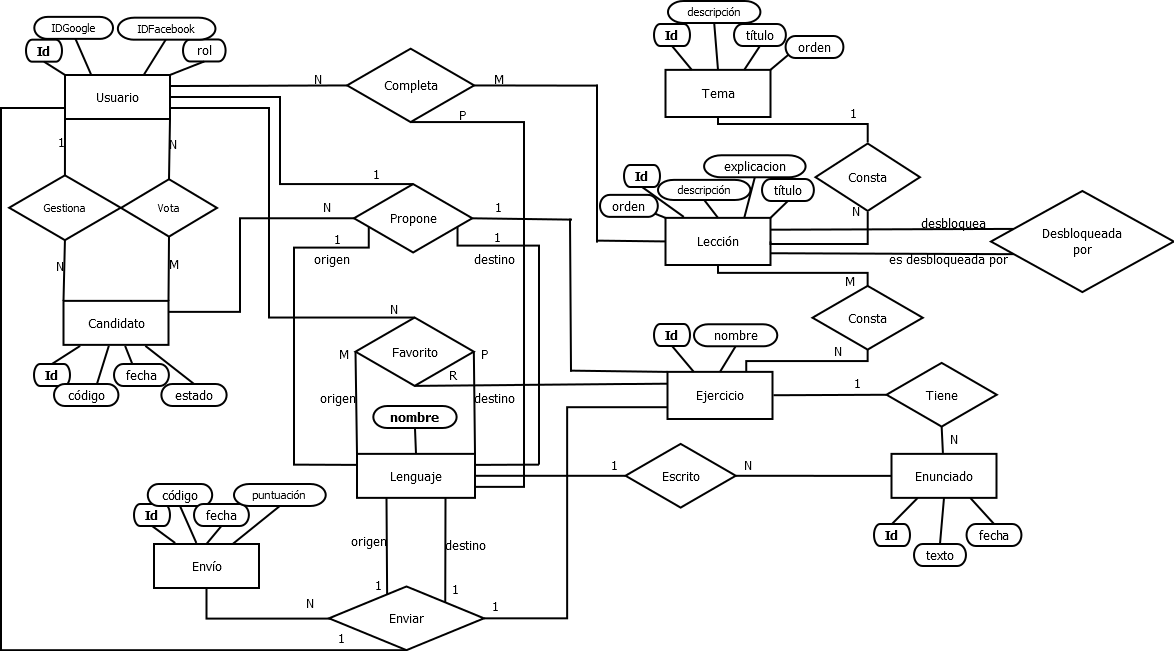
\includegraphics[width=\paperwidth]{images/bd-tfg}}
\caption{Modelo entidad-relacion\label{fig:ent_rel}}
\end{center}
\end{sidewaysfigure}

\begin{figure}
\begin{center}
\makebox[\textwidth]{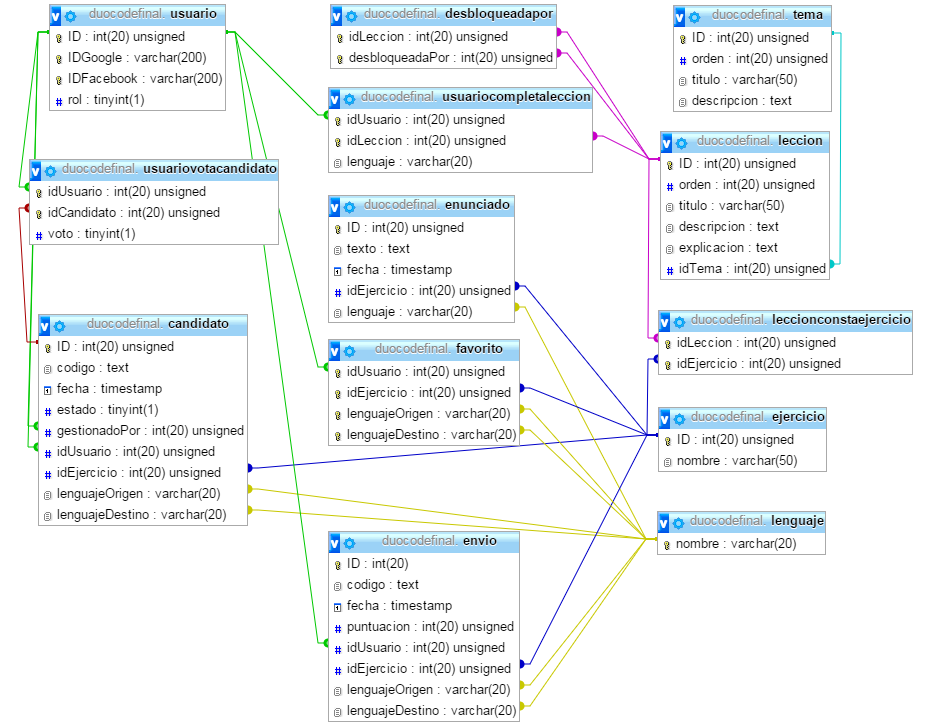
\includegraphics[scale=0.7]{images/bd}}
\caption{Modelo relacional\label{fig:rel}}
\end{center}
\end{figure}

\newpage

\textbf{Estructura de las tablas}

\begin{itemize}
\item Usuario: Tabla que contiene los datos de los usuarios. No hace falta guardar el nombre u otros datos personales ya que los obtenemos de la aplicación con la que haya iniciado sesión.


\begin{tabularx}{14cm}{|l|X|}
\hline
\textbf{Nombre} & \textbf{Descripción}                                                              \\ \hline
ID              & ID que le asigna la aplicación al usuario.                                         \\ \hline
IDGoogle        & ID que le asigna Google. Es opcional ya que el usuario puede iniciar con Facebook. \\ \hline
IDFacebook      & ID que le asigna Facebook. Es opcional ya que el usuario puede iniciar con Google. \\ \hline
\end{tabularx}
\vspace{1em}

\item UsuarioVotaCandidato: Tabla que contiene todos los votos de los usuarios a los candidatos.

\begin{tabularx}{14cm}{|l|X|}
\hline
\textbf{Nombre} & \textbf{Descripción}                                                              \\ \hline
IDUsuario       & ID del usuario que vota.                                                           \\ \hline
IDCandidato     & ID del candidato al que se quiere votar.                                           \\ \hline
Voto            & Puede tomar los valores 0 o 1 dependiendo de si el voto es positivo (1) o negativo (0). \\ \hline
\end{tabularx}
\vspace{1em}

\item Candidato: Tabla que contiene la información de los candidatos enviados por los usuarios de la aplicación.

\begin{tabularx}{14cm}{|l|X|}
\hline
\textbf{Nombre} & \textbf{Descripción}                                                              \\ \hline
ID              & Identificador único para el candidato.                                         \\ \hline
Código        & Texto propuesto como posible solución del ejercicio. \\ \hline
Fecha      & Fecha en la que se realiza la propuesta. \\ \hline
Estado              & Puede ser No Gestionado (0), Aceptado (1) o Rechazado (-1).                                         \\ \hline
GestionadoPor        & ID del usuario administrador que finalmente acepta o rechaza el candidato. Inicialmente se encuentra vacío. \\ \hline
IDUsuario      & ID del usuario que propone el candidato. \\ \hline
IDEjercicio              & ID del ejercicio que resuelve dicho candidato.                                         \\ \hline
LenguajeOrigen        & Lenguaje en el que se encuentra el enunciado del ejercicio. \\ \hline
LenguajeDestino      & Lenguaje en el que está la posible solución. \\ \hline
\end{tabularx}
\vspace{1em}

\item Tema: Tabla que contiene la información de los temas, primera división para organizar los ejercicios según a qué van dedicados. Los temas se conforman de una colección de lecciones.

\begin{tabularx}{14cm}{|l|X|}
\hline
\textbf{Nombre} & \textbf{Descripción}                                                              \\ \hline
ID       & ID propio del tema                                                           \\ \hline
Orden     & Orden en el que queremos que aparezca el tema.                                           \\ \hline
Título            & Nombre que distingue a los temas. \\ \hline
Descripción            & Texto breve que describe el tema. \\ \hline
\end{tabularx}
\vspace{1em}

\item Lección: Tabla que contiene la información de las lecciones, segunda división para la organización. Las lecciones se conforman de una serie de ejercicios y están incluidas en temas.

\begin{tabularx}{14cm}{|l|X|}
\hline
\textbf{Nombre} & \textbf{Descripción}                                                              \\ \hline
ID              & Identificador único para la lección.                                         \\ \hline
Orden        & Orden en el que queremos que aparezca la lección. \\ \hline
Título      & Nombre que distingue a las lecciones. \\ \hline
Descripción              & Texto breve que describe la lección.                                         \\ \hline
Expliciación        & Texto largo que sirve como introducción a la lección.  \\ \hline
IDTema      & ID del tema al que pertenece esta lección. \\ \hline
\end{tabularx}
\vspace{1em}

\item UsuarioCompletaLeccion: Tabla que contiene la relación de las lecciones con los usuarios que las han completado.

\begin{tabularx}{14cm}{|l|X|}
\hline
\textbf{Nombre} & \textbf{Descripción}                                                              \\ \hline
IDUsuario       & ID del usuario que ha completado la lección.                                                          \\ \hline
IDLección     & Lección que ha sido completada.                                           \\ \hline
Lenguaje            & Lenguaje en el que se ha completado dicha lección, ya que una lección puede ser completada por el mismo usuario en distintos lenguajes. \\ \hline
\end{tabularx}
\vspace{1em}

\item DesbloqueadaPor: Tabla que contiene la dependencia entre lecciones. Hay lecciones a las que solo se puede acceder si se han superado otras anteriormente.

\begin{tabularx}{14cm}{|l|X|}
\hline
\textbf{Nombre} & \textbf{Descripción}                                                              \\ \hline
IDLección       & ID de la lección a la que queremos asignar dependencia.                                                          \\ \hline
DesbloqueadaPor     & Lección que debe ser superada para poder acceder a la mencionada anteriormente.                                           \\ \hline
Lenguaje            & Lenguaje en el que se ha completado dicha lección, ya que una lección puede ser completada por el mismo usuario en distintos lenguajes. \\ \hline
\end{tabularx}
\vspace{1em}

\item Ejercicio: Tabla que contiene la información de los ejercicios existentes.

\begin{tabularx}{14cm}{|l|X|}
\hline
\textbf{Nombre} & \textbf{Descripción}                                                              \\ \hline
ID       & Identificador asignado por la aplicación para cada ejercicio. \\ \hline
Nombre     & Nombre con el que se diferenciará de los demás.                                           \\ \hline
\end{tabularx}
\vspace{1em}

\item LeccionConstaEjercicio: Tabla que contiene la relación donde se asignan los ejercicios a las correspondientes lecciones.

\begin{tabularx}{14cm}{|l|X|}
\hline
\textbf{Nombre} & \textbf{Descripción}                                                              \\ \hline
IDLección       & ID de la lección a la que se añade un ejercicio. \\ \hline
IDEjercicio     & ID del ejercicio añadido a la lección.                                           \\ \hline
\end{tabularx}
\vspace{1em}

\item Lenguaje: Tabla que contiene los lenguajes que podrán aprender los usuarios.

\begin{tabularx}{14cm}{|l|X|}
\hline
\textbf{Nombre} & \textbf{Descripción}                                                              \\ \hline
Nombre       & Nombre del lenguaje. \\ \hline
\end{tabularx}
\vspace{1em}

\item Enunciado: Tabla que contiene la información de los enunciados. Un enunciado es un código con un correspondiente lenguaje que forma parte de un ejercicio. Un ejercicio puede tener varios enunciados en varios idiomas.

\begin{tabularx}{14cm}{|l|X|}
\hline
\textbf{Nombre} & \textbf{Descripción}                                                              \\ \hline
ID       & ID que identifica al enunciado. \\ \hline
Texto     & Código, en lenguaje de origen, que tendrá que ser \emph{traducido}.                                           \\ \hline
Fecha     & Fecha en la que fue añadido el enunciado.                                           \\ \hline
IDEjercicio     & ID del ejercicio al que corresponde este enunciado.                                           \\ \hline
Lenguaje     & Lenguaje en el que está escrito el código de dicho enunciado.                                           \\ \hline
\end{tabularx}
\vspace{1em}

\item Favorito: Tabla que contiene la relación entre los usuarios y los ejercicios favoritos de estos.

\begin{tabularx}{14cm}{|l|X|}
\hline
\textbf{Nombre} & \textbf{Descripción}                                                              \\ \hline
IDUsuario       & ID del usuario que añade un ejercicio a favorito. \\ \hline
IDEjercicio     & ID del ejercicio que ha sido marcado como favorito. \emph{traducido}                                           \\ \hline
LenguajeOrigen     & Lenguaje del enunciado que ha sido marcado como favorito.                                           \\ \hline
LenguajeDestino     & Lenguaje que el usuario quería aprender al marcar este ejercicio como favorito.                                           \\ \hline
\end{tabularx}
\vspace{1em}

\item Envío: Tabla que contiene la relación entre los usuarios y todos los ejercicios que han realizado en la aplicación.

\begin{tabularx}{14cm}{|l|X|}
\hline
\textbf{Nombre} & \textbf{Descripción}                                                              \\ \hline
ID       & ID correspondiente a cada envío. \\ \hline
Código     & Código respuesta del usuario. \emph{traducido}                                           \\ \hline
Fecha     & Fecha en la que se ha resuelto el ejercicio.                                           \\ \hline
Puntuación     & Puntuación obtenida.                                           \\ \hline
IDUsuario     & Usuario que ha realizado el envío.                                           \\ \hline
IDEjercicio     & Ejercicio resuelto.                                           \\ \hline
LenguajeOrigen     & Lenguaje inicial del enunciado.                                           \\ \hline
LenguajeDestino     & Lenguaje en el que el usuario ha enviado el ejercicio.                                           \\ \hline
\end{tabularx}

\end{itemize}

\newpage
\section{Manual de usuario\label{sec:manual}}
%!TEX root = memoria_duocode_interfaz.tex

En esta sección se muestra el funcionamiento de la aplicación web desde el punto de vista de un usuario.

\subsection{Lenguajes}
Al acceder al inicio de la web se nos muestran un par de listas con lenguajes de programación, donde podremos elegir cuál sabemos y cuál queremos aprender, en ningún caso será posible elegir la misma opción en ambos lados. En la parte superior se encuentra la barra de navegación que estará accesible en todo momento.

\begin{figure}[H]
\begin{center}
\makebox[\textwidth]{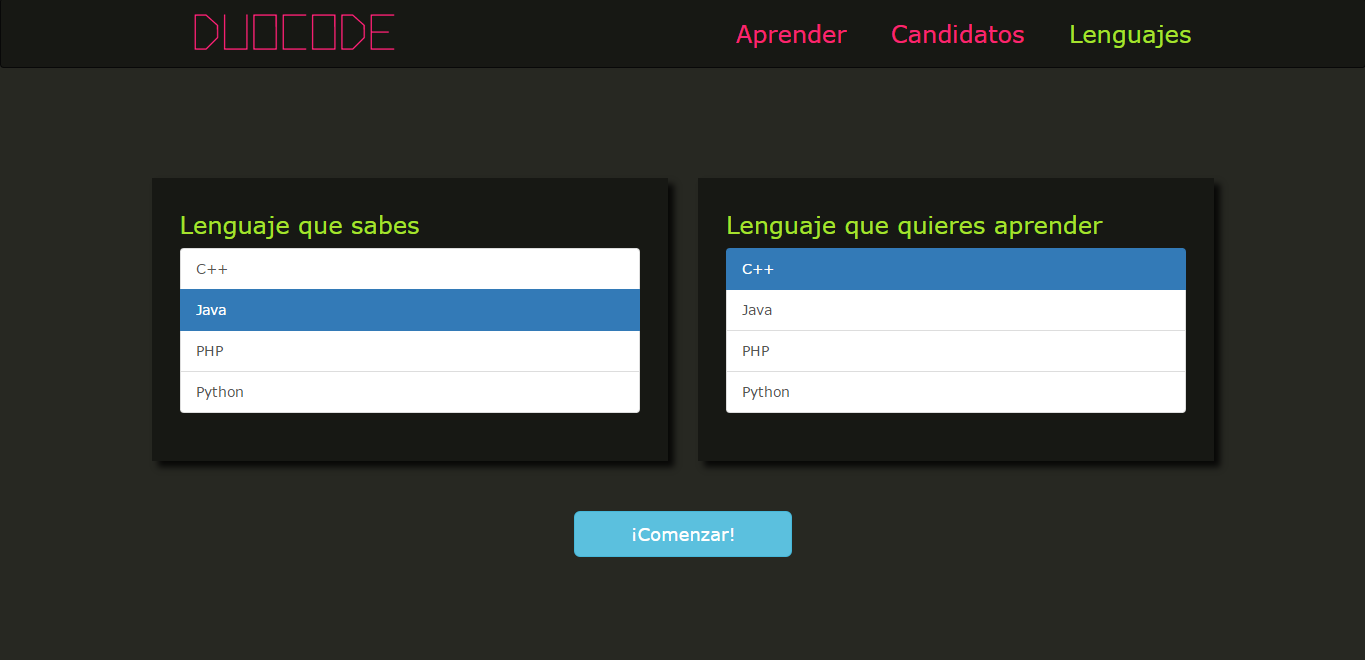
\includegraphics[scale=0.4]{images/lenguajes}}
\caption{Lenguajes\label{fig:lenguajes}}
\end{center}
\end{figure}

Una vez pulsado el botón de ``¡Comenzar!'', pasamos a la página de los temas.

\subsection{Temas}
En esta sección nos encontramos con dos partes diferenciadas. Por una parte, tenemos el login/información de usuario y por otra todos los temas disponibles con una breve explicación sobre estos.

\begin{figure}[H]
\begin{center}
\makebox[\textwidth]{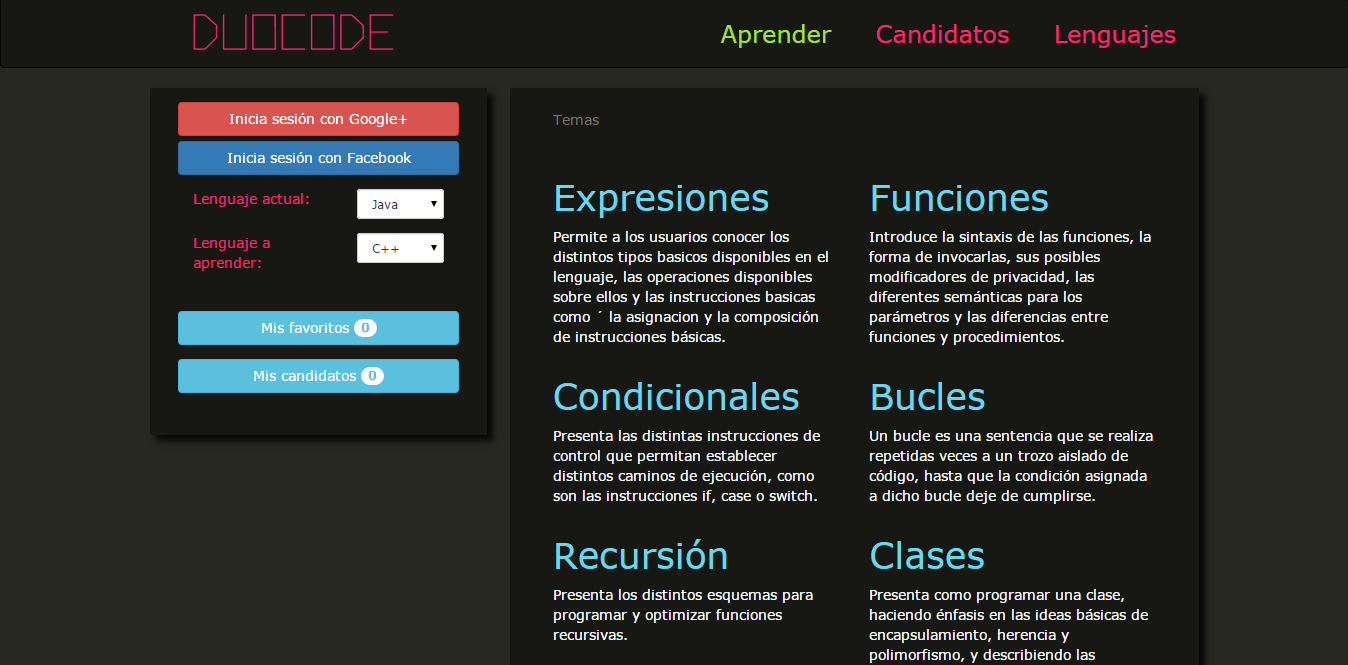
\includegraphics[scale=0.4]{images/temas}}
\caption{Temas\label{fig:temas}}
\end{center}
\end{figure}

Tenemos la posibilidad de iniciar sesión tanto con Google como con Facebook.

\begin{figure}[H]
\begin{center}
\makebox[\textwidth]{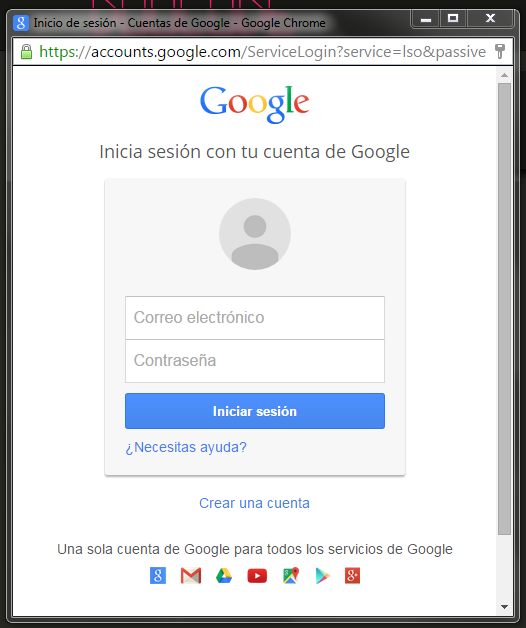
\includegraphics[scale=0.6]{images/Google}}
\caption{Inicio de sesión con Google\label{fig:google}}
\end{center}
\end{figure}

\begin{figure}[H]
\begin{center}
\makebox[\textwidth]{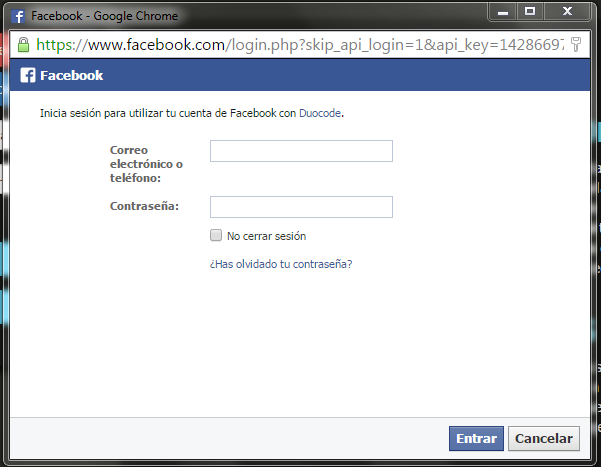
\includegraphics[scale=0.6]{images/Facebook}}
\caption{Inicio de sesión con Facebook\label{fig:facebook}}
\end{center}
\end{figure}

En ambos casos se pedirá permiso al usuario para acceder a su información de perfil. Después de iniciar sesión, en la información de usuario aparecerá el nombre y la imagen de su perfil de red social, su puntuación total en DuoCode, los lenguajes seleccionados anteriormente, su número de ejercicios favoritos y candidatos enviados en la aplicación. 

\begin{figure}[H]
\begin{center}
\makebox[\textwidth]{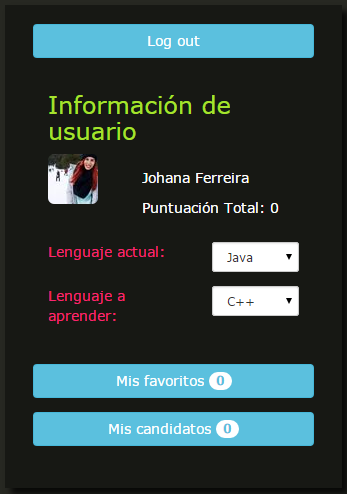
\includegraphics[scale=0.6]{images/usuario}}
\caption{Información de usuario\label{fig:usuario}}
\end{center}
\end{figure}

Una vez seleccionado un tema, pasamos a las lecciones.

\subsection{Lecciones}

Al seleccionar un tema accedemos a sus correspondientes lecciones, de las cuales podemos ver un pequeño resumen. Si el nombre de la lección aparece en blanco significa que ésta es dependiente de otra, es decir, tienes que superar antes otra lección para poder acceder a ésta.

\begin{figure}[H]
\begin{center}
\makebox[\textwidth]{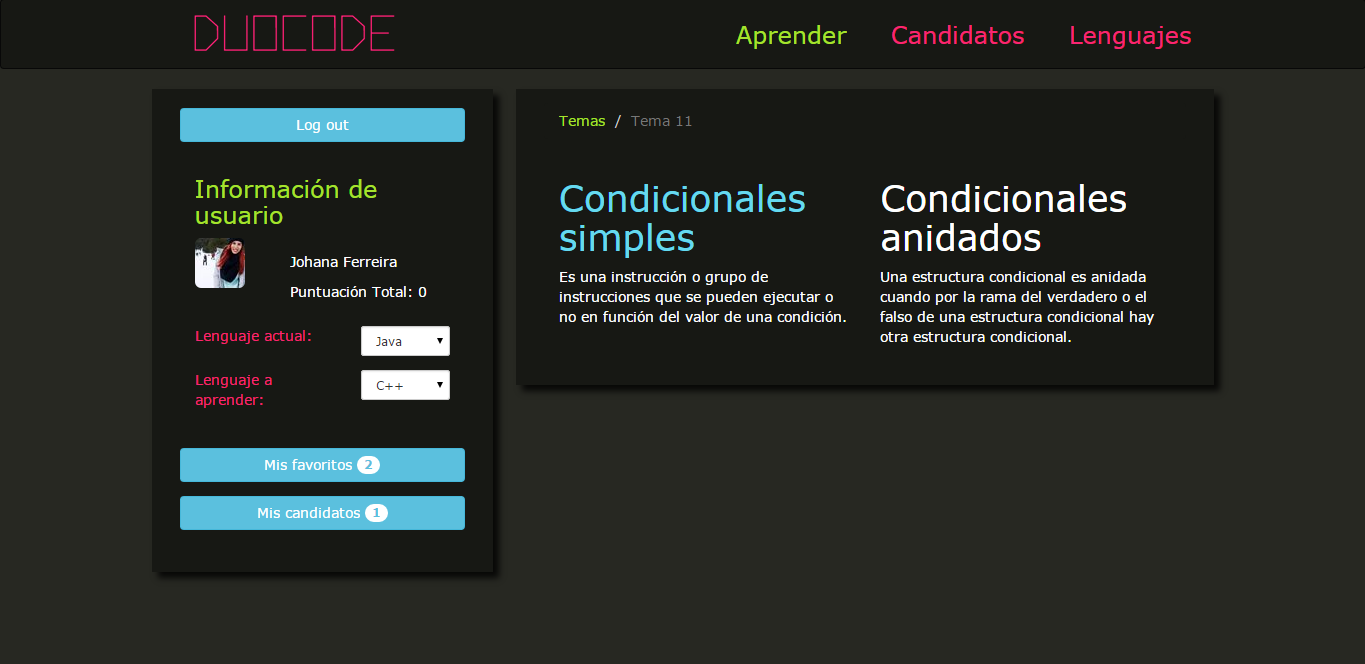
\includegraphics[scale=0.4]{images/lecciones}}
\caption{Lecciones\label{fig:lecciones}}
\end{center}
\end{figure}

Una vez seleccionada una lección, pasamos a los ejercicios.

\subsection{Ejercicios}

En esta parte lo primero que nos encontramos es un pop-up con una explicación de la lección, al que se podrá acceder nuevamente a lo largo de ésta. 

\begin{figure}[H]
\begin{center}
\makebox[\textwidth]{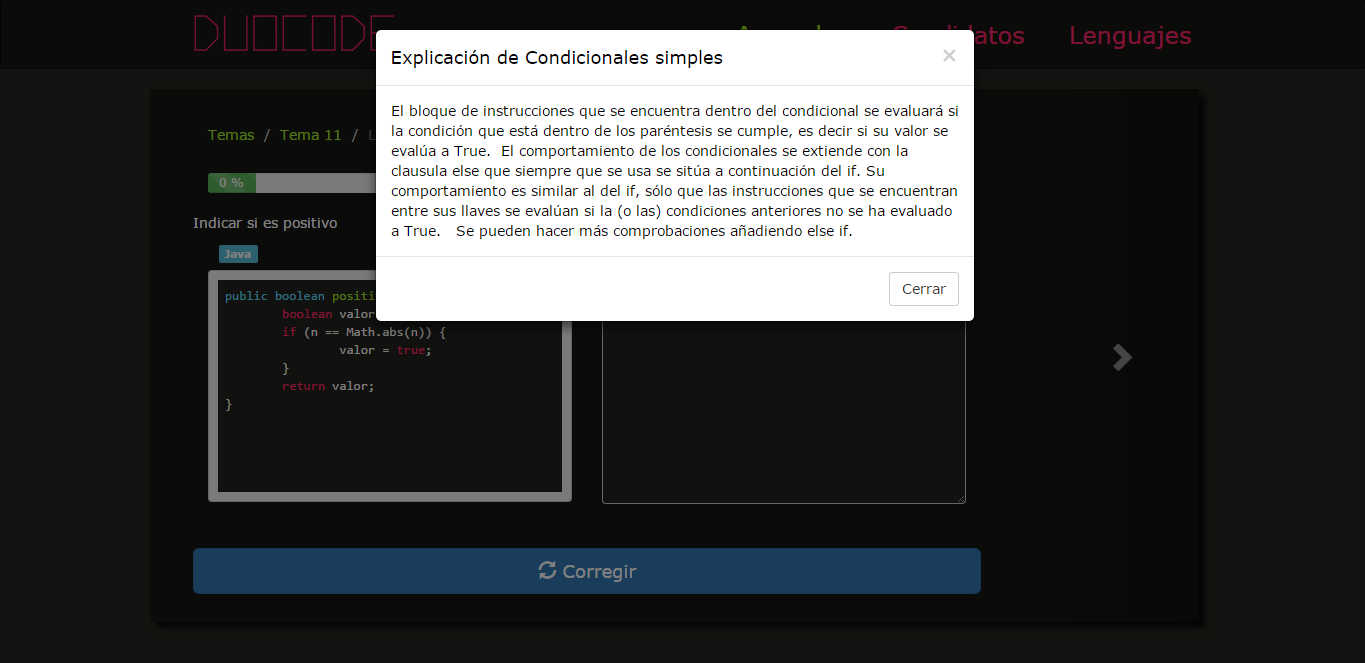
\includegraphics[scale=0.4]{images/popup}}
\caption{Pop-up al iniciar una lección\label{fig:popup}}
\end{center}
\end{figure}

Al cerrar el pop-up empezamos con los ejercicios. En todo momento encontramos varios elementos en la parte superior: una barra en la que se indica el porcentaje que se ha completado de la lección, las vidas restantes, un botón para añadir a favorito el ejercicio actual y un botón de ayuda con el que se muestra el pop-up del principio.

\vspace{1em}

Para cada ejercicio se muestra su título y dos cuadros de código, uno con el del enunciado del ejercicio y otro vacío que es donde el usuario tendrá que resolver el ejercicio.

\vspace{1em}

Por último está el botón de ``Corregir'' con el cual enviamos el ejercicio a ser corregido.

\begin{figure}[H]
\begin{center}
\makebox[\textwidth]{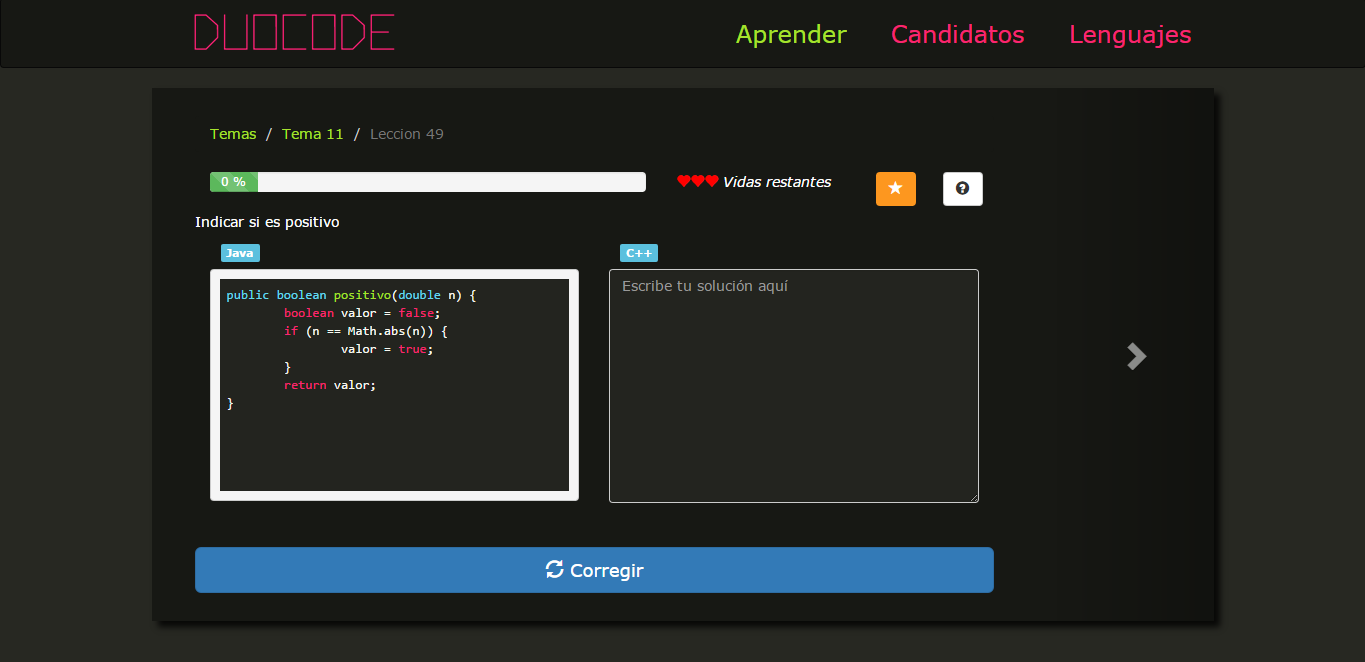
\includegraphics[scale=0.4]{images/ejercicio}}
\caption{Ejercicio\label{fig:ejercicio}}
\end{center}
\end{figure}

Después de corregir el ejercicio hay dos posibilidades:
\begin{itemize}
\item[•]Solución correcta: En este caso se muestra un mensaje con la puntuación obtenida.

\begin{figure}[H]
\begin{center}
\makebox[\textwidth]{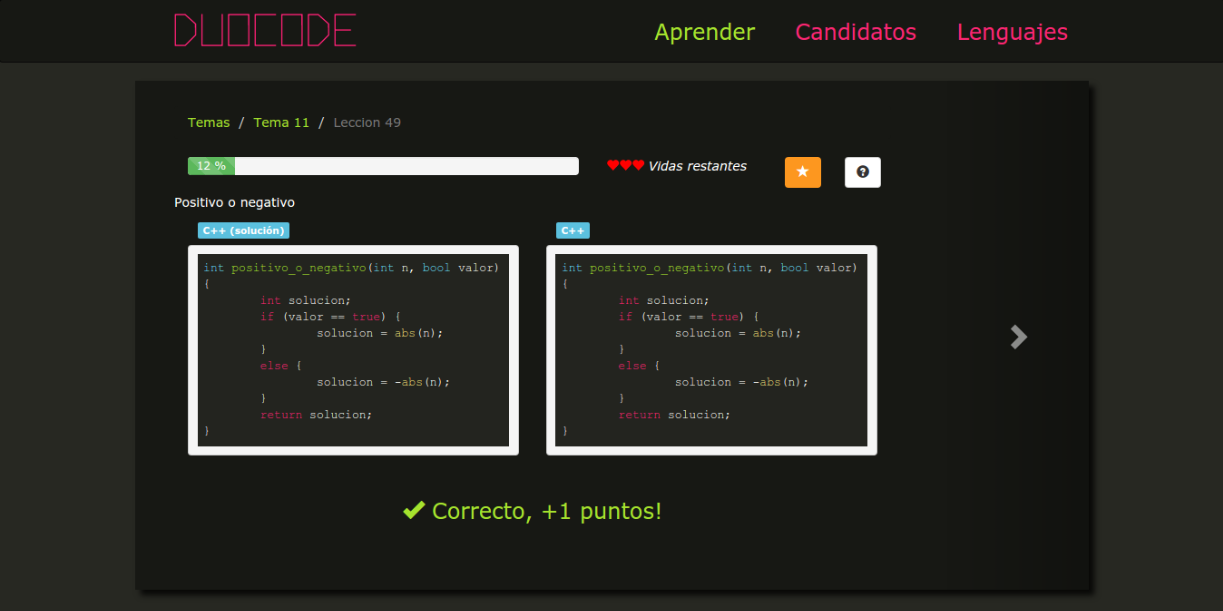
\includegraphics[scale=0.45]{images/ejercicioCorrecto}}
\caption{Ejercicio correcto\label{fig:correcto}}
\end{center}
\end{figure}

\item[•]Solución incorrecta: En este caso se resta un corazón, se muestra un mensaje de incorrecto y la puntuación obtenida. Donde estaban anteriormente el código de enunciado y la solución del usuario, ahora se muestra el enunciado y la solución correcta. También se da la posibilidad al usuario de enviar su ejercicio como candidato si piensa que la solución que dio era correcta y si el usuario no sabe qué son los candidatos se encuentra también un botón con un pop-up explicativo.

\begin{figure}[H]
\begin{center}
\makebox[\textwidth]{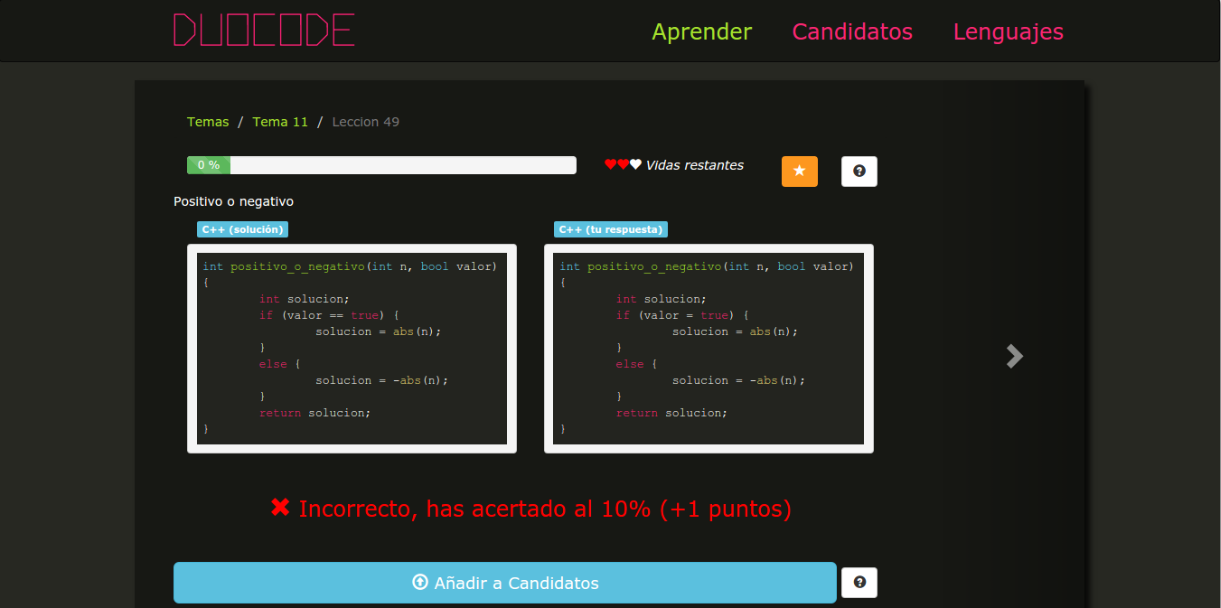
\includegraphics[scale=0.45]{images/ejercicioIncorrecto}}
\caption{Información de usuario\label{fig:usuario}}
\end{center}
\end{figure}

\begin{figure}[H]
\begin{center}
\makebox[\textwidth]{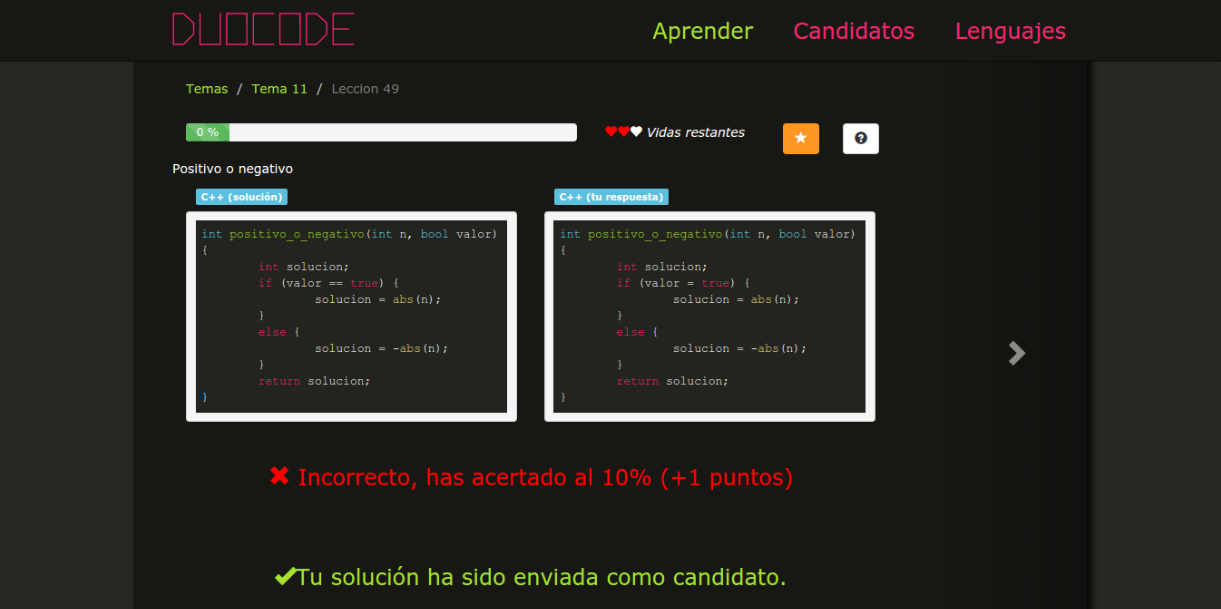
\includegraphics[scale=0.45]{images/enviarCandidato}}
\caption{Información de usuario\label{fig:usuario}}
\end{center}
\end{figure}

\end{itemize}

Hay dos posibilidades de acabar las lecciones:

\begin{itemize}

\item[•]Sin vidas: Una lección puede acabar si se acaban los corazones de los que dispone el usuario, es decir, si falla tres veces. Se muestra un botón mediante el cual el usuario puede volver a intentar la misma lección.

\begin{figure}[H]
\begin{center}
\makebox[\textwidth]{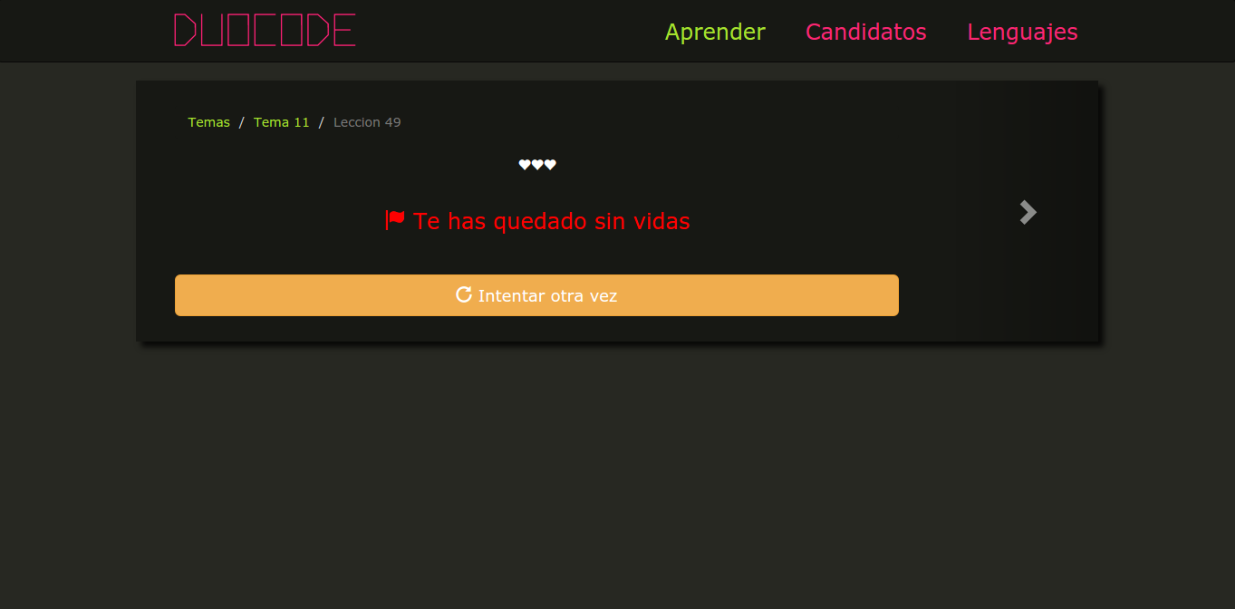
\includegraphics[scale=0.45]{images/sinVidas}}
\caption{Información de usuario\label{fig:usuario}}
\end{center}
\end{figure}

\item[•]Lección completada: Al acabar la lección con vidas, ésta se da como superada y se da la opción de compartir en Facebook el resultado. A partir de aquí podemos volver a las lecciones para seguir aprendiendo.

\begin{figure}[H]
\begin{center}
\makebox[\textwidth]{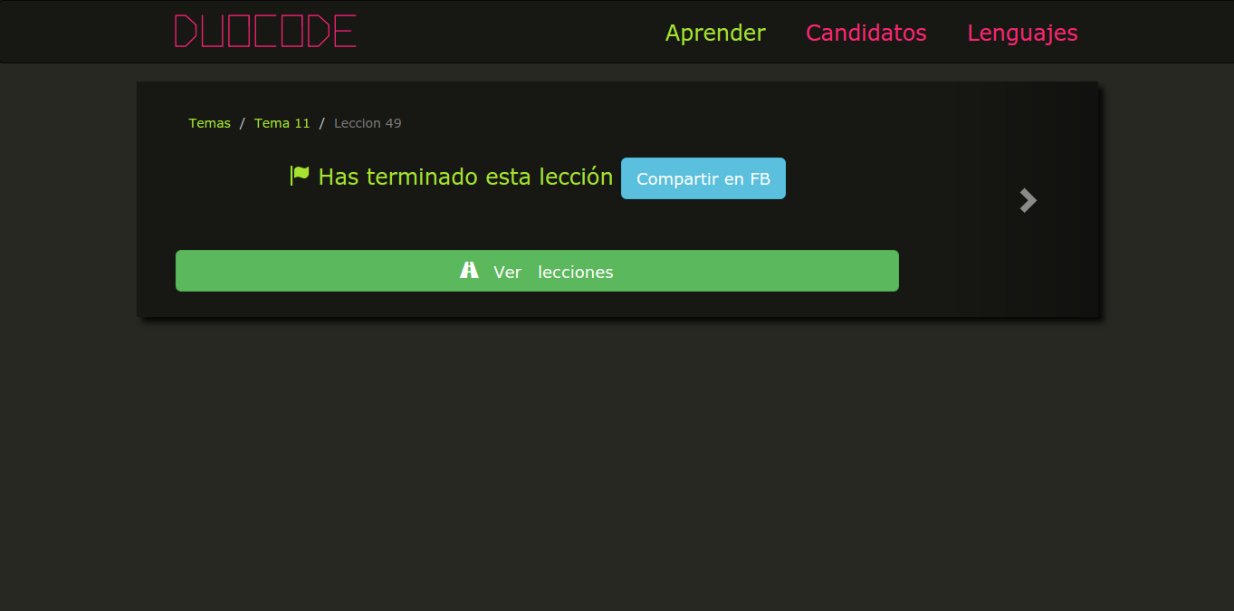
\includegraphics[scale=0.45]{images/leccionCompletada}}
\caption{Información de usuario\label{fig:usuario}}
\end{center}
\end{figure}

\begin{figure}[H]
\begin{center}
\makebox[\textwidth]{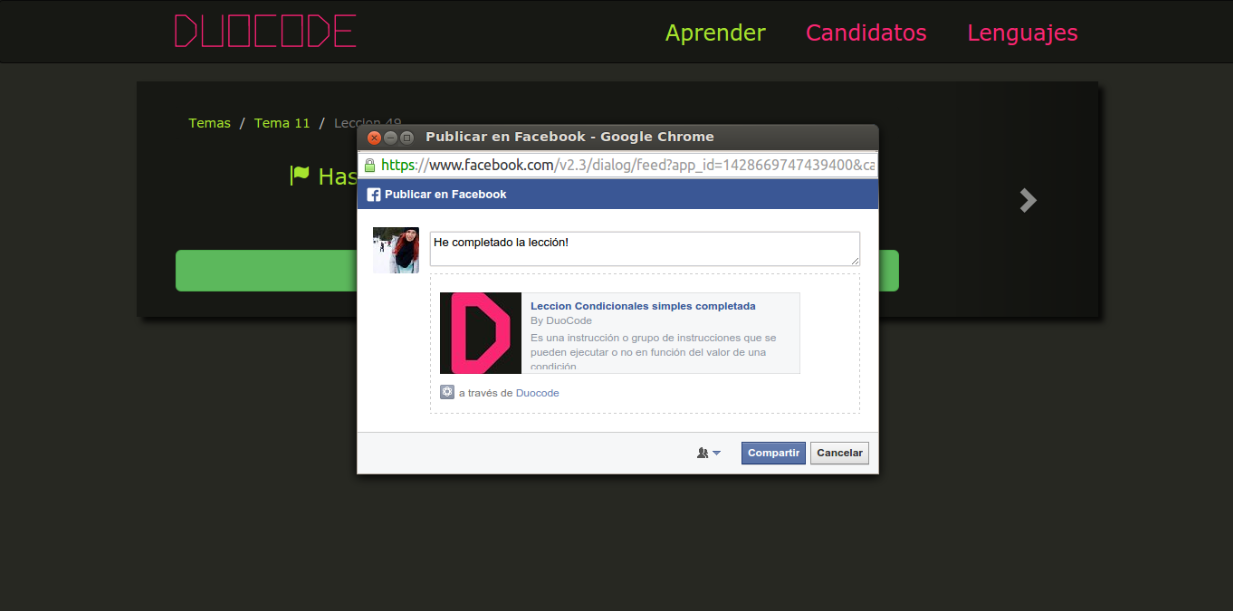
\includegraphics[scale=0.45]{images/compartirFB}}
\caption{Información de usuario\label{fig:usuario}}
\end{center}
\end{figure}

\end{itemize}

\subsection{Mis favoritos}

Desde la información de usuario se puede acceder a los favoritos del usuario.

\vspace{1em}

De cada ejercicio se muestra su título, los lenguajes que estaban seleccionados al marcar el ejercicio como favorito y un botón que al seleccionarlo muestra los códigos de origen y destino y la opción de desmarcarlo como favorito.

\begin{figure}[H]
\begin{center}
\makebox[\textwidth]{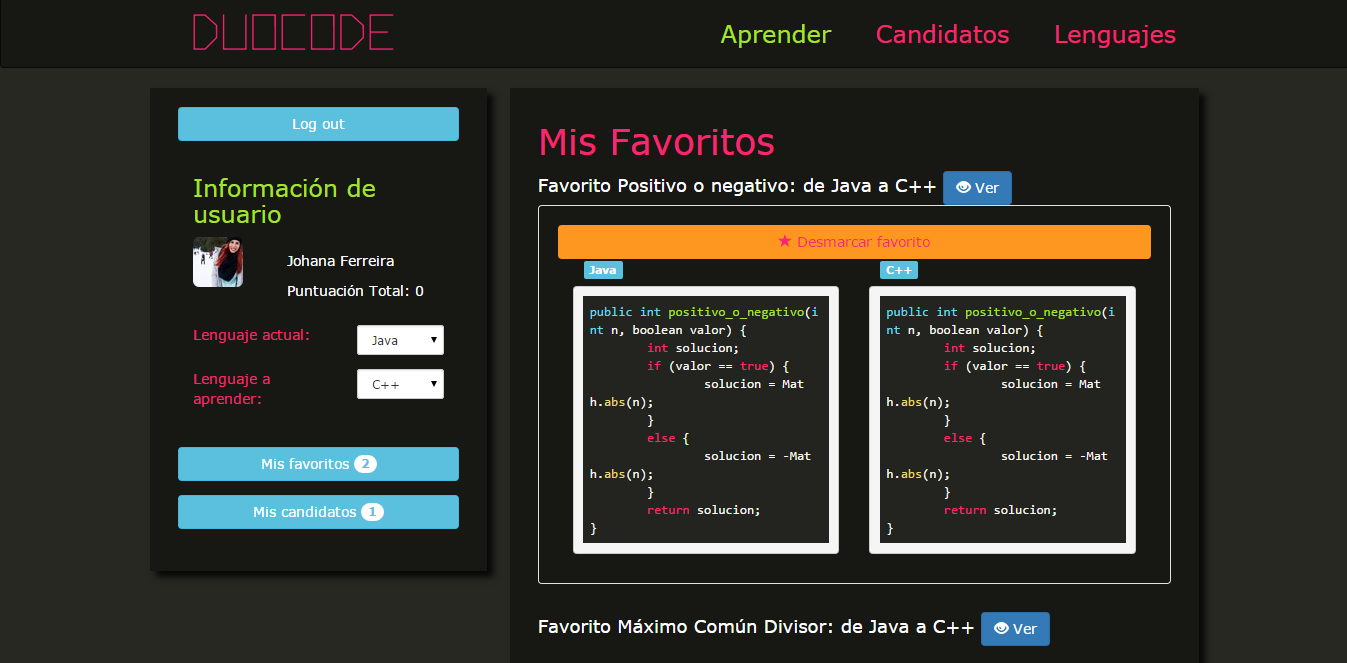
\includegraphics[scale=0.4]{images/favoritos}}
\caption{Información de usuario\label{fig:usuario}}
\end{center}
\end{figure}

\subsection{Mis candidatos}

Desde la información de usuario se puede acceder a los candidatos del usuario.

\vspace{1em}

De cada ejercicio se muestra su título, los lenguajes que estaban seleccionados al enviar el ejercicio como candidato y un botón que al seleccionarlo muestra el código del enunciado, la solución propuesta por el usuario y la opción de eliminar dicho candidato. Si el candidato ha sido aceptado o rechazado se indica en la parte superior.

\begin{figure}[H]
\begin{center}
\makebox[\textwidth]{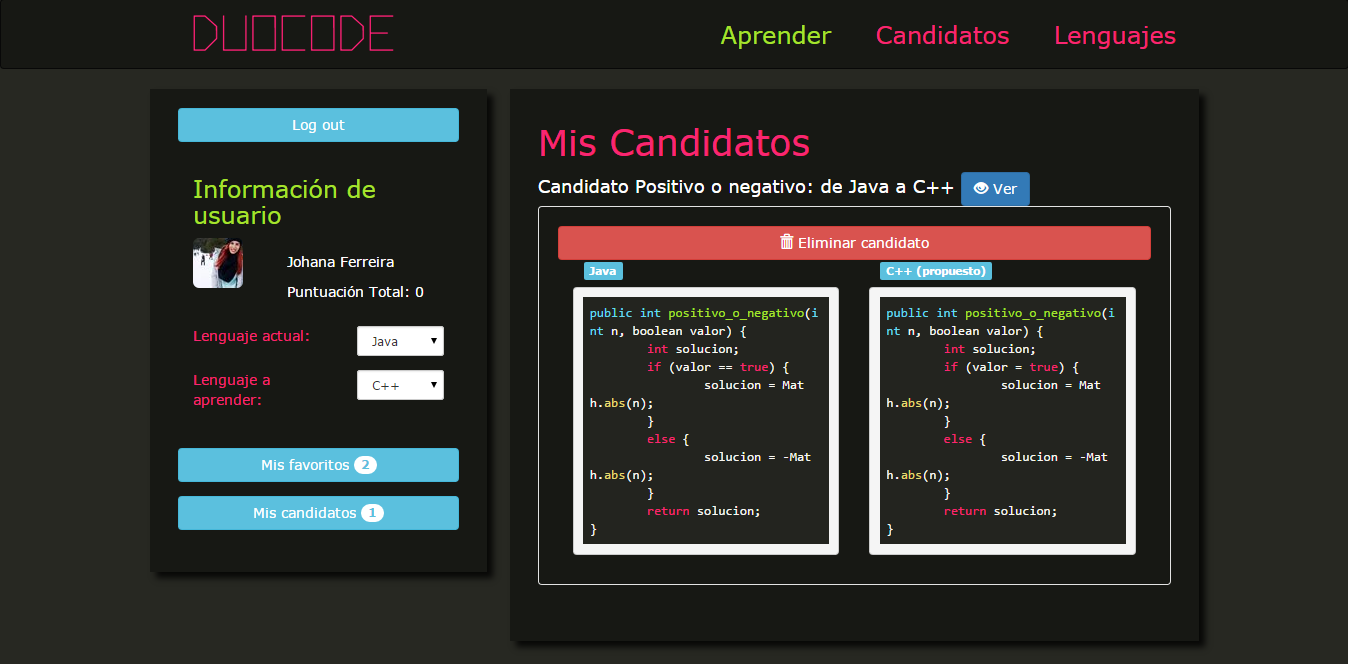
\includegraphics[scale=0.4]{images/misCandidatos}}
\caption{Información de usuario\label{fig:usuario}}
\end{center}
\end{figure}

\subsection{Candidatos}

Desde la barra de navegación tenemos acceso al apartado ``Candidatos'' en el cual se muestran los candidatos propuestos por los demás usuarios. De cada uno se muestra una barra con la cantidad de votos positivos y negativos que ha recibido, el nombre del ejercicio, el código del enunciado, el código propuesto a evaluación y dos botones en los que se puede votar si se está de acuerdo o no.

\begin{figure}[H]
\begin{center}
\makebox[\textwidth]{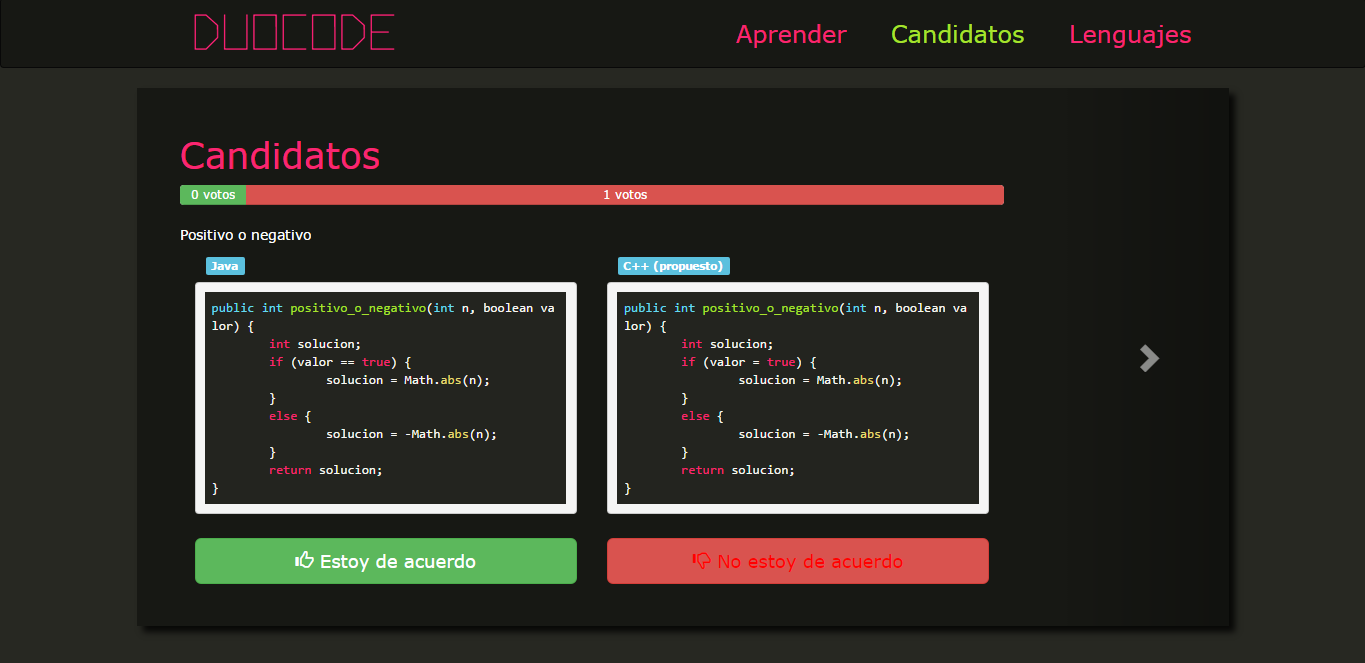
\includegraphics[scale=0.4]{images/candidatos}}
\caption{Información de usuario\label{fig:usuario}}
\end{center}
\end{figure}

Además, si el usuario es administrador se muestran otros dos botones adicionales mediante los cuales se acepta o rechaza un candidato definitivamente. Si se acepta pasa a ser solución válida del ejercicio, si se rechaza se elimina, en cualquiera de los casos ya no se encontraría en la lista de candidatos para evaluar.

\begin{figure}[H]
\begin{center}
\makebox[\textwidth]{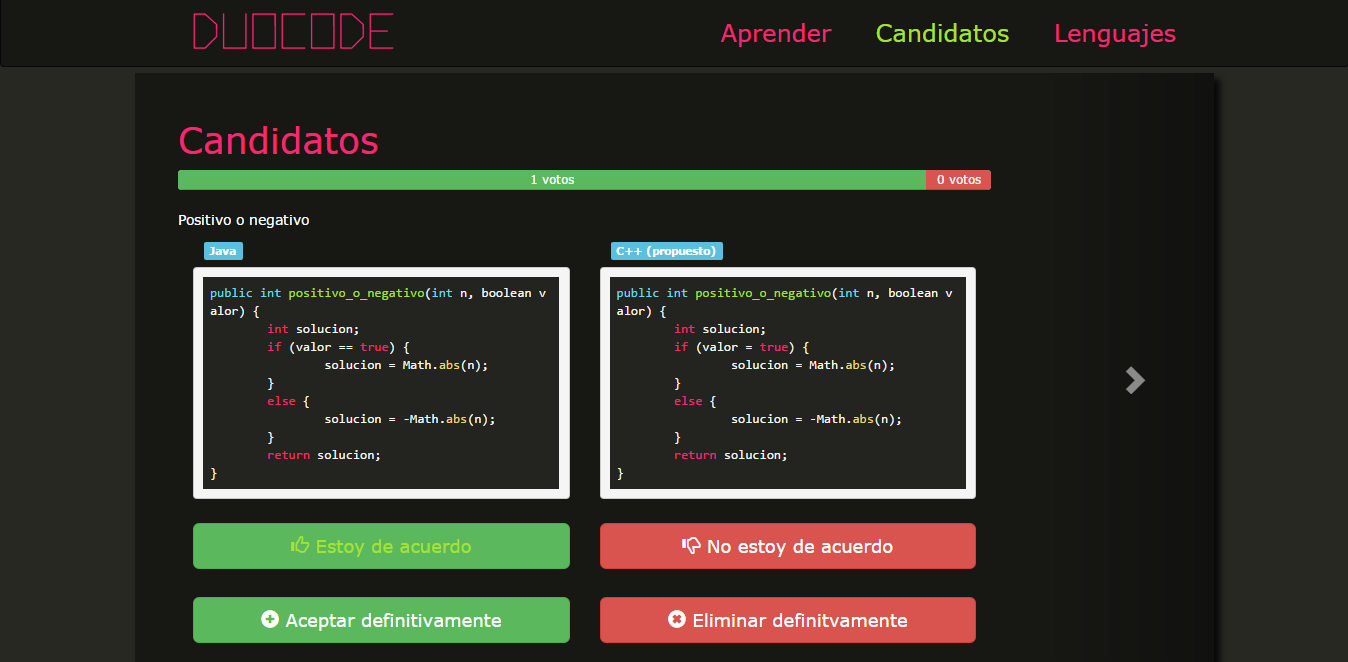
\includegraphics[scale=0.4]{images/candidatosAdmin}}
\caption{Información de usuario\label{fig:usuario}}
\end{center}
\end{figure}

Si ya se han evaluado todos los candidatos existentes se muestra un mensaje al usuario informándole de ello y un botón que le dirige a los temas para que siga aprendiendo.

\begin{figure}[H]
\begin{center}
\makebox[\textwidth]{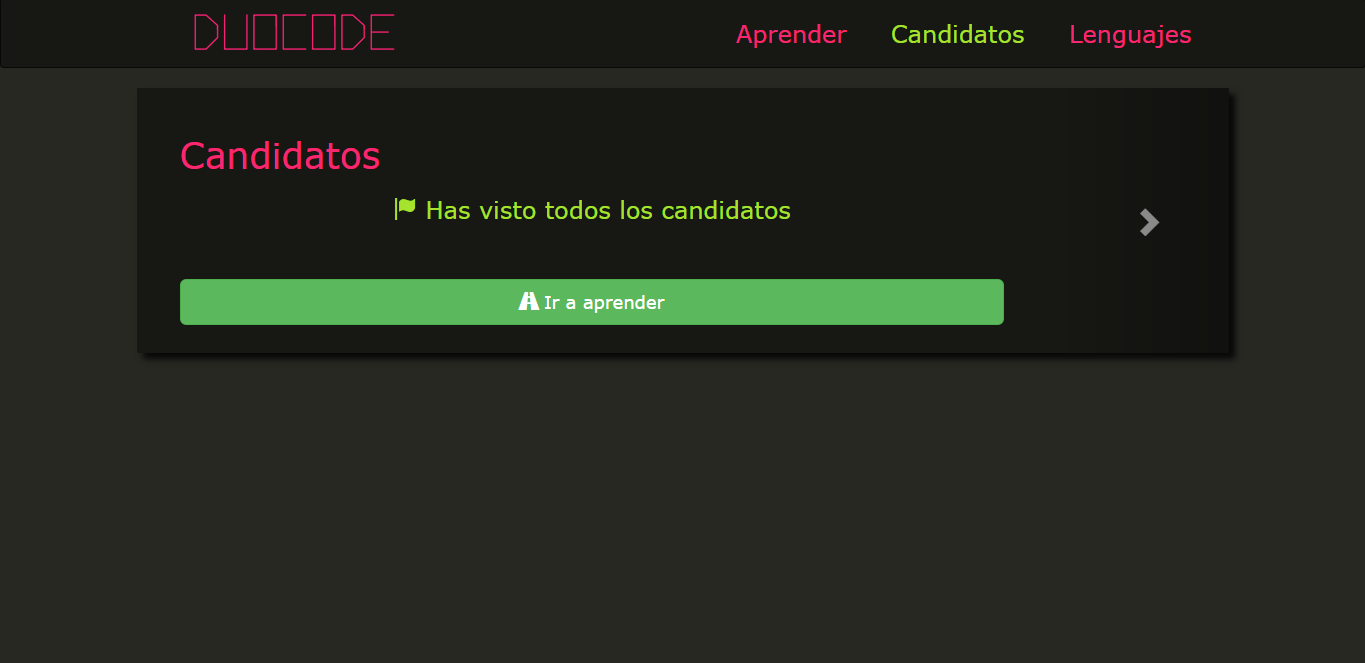
\includegraphics[scale=0.4]{images/sinCand}}
\caption{Información de usuario\label{fig:usuario}}
\end{center}
\end{figure}

\newpage
\section{Conclusiones\label{sec:conc}}
ñasñlkjñjk

\newpage
\section{Conclusions\label{sec:concEn}}
%!TEX root = memoria_duocode_interfaz.tex

In this project we have developed \textit{DuoCode}, a new way for learning how to code. It consists of a platform where users can learn new programming languages by translating small pieces of code from a known one. It can even be the natural language if the user has never studied any programming language before.

During our years in the university we have acquired knowledge about different areas related to computer science. Developing \textit{DuoCode} allowed us to apply all our knowledge into a single project. Moreover, we also learned new technologies that helped us growing as engineers, such as \textit{AngularJS}, \textit{BootStrap}, \textit{Jersey} or \textit{PhoneGap}.

First of all we decided to use an agile development methodology. Every sprint lasted 2 weeks and ended with a meeting where we talked about what we did. It was a new way of developing for us; we were used to apply traditional methodologies such as \textit{Waterfall} or \textit{Spiral Development}. It was a great decision, since we have had very good results and we have learned how to use one of the most popular ways of development nowadays.

We have also learned how to work in team by using \textit{Git}, the most common distributed version control. It took us some weeks to learn \textit{Git}, it is not simple and has a lot of features.
However, it was very useful once we learned how to use the basic commands.

We had a lot of problems trying to configure SSL on \textit{GlassFish} in order to use \texttt{HTTPS} protocol. It was probably the task that took most of our time so we decided to switch to \textit{TomCat}. \textit{TomCat} is similar to \textit{GlassFish} but it has much more documentation. Finally, we could configure the server to use the \texttt{HTTPS} protocol.

We are proud of the final result. We have learned new technologies and \textit{DuoCode} is a good way for future students to learn the basics of coding in a new language. Nowadays a lot of schools are interested in teaching how to code. \textit{DuoCode} is a very useful platform where students can practice and apply their knowledge.

\textit{DuoCode} constitutes a good base for future extensions, so it can be extended on many ways. We have used design patterns such as \textit{Abstract Mapper} or \textit{AngularJS} framework to obtain a maintainable code, making it easier to future developers to extend their project. Although the actual version of \textit{DuoCode} is stable, a lot of new features can be implemented:

\begin{itemize}
\item Integrate \textit{Open Badges}: a new online standard to recognize and verify learning. More info can be found at \url{http://openbadges.org/}

\item Show which parts of the code are wrong.

\item Intercalate questions in different languages.

\item Group languages with same programming paradigm.

\item Highlight syntax in real time.

\item Allow the user to change the interface colors.

\item Improve the mobile version.

\item Implement database normalization.

\end{itemize}

\newpage
\section{Tareas de Julián F. Calleja da Silva\label{sec:julian}}
%!TEX root = memoria_duocode_interfaz.tex

Todos nos hemos ayudado y colaborado durante este proyecto pero en esta sección explicaré las tareas que yo, Julián~F. Calleja da~Silva, específicamente he realizado.

\begin{itemize}
\item
Cuando investigamos los diferentes enfoques para realizar servicios web, me encargué de SOAP, vi sus ventajas y desventajas e incluso hice un pequeño ejemplo para entender mejor su funcionamiento.

\item
Hicimos una reunión para ponernos de acuerdo en cual era el mejor enfoque para el servicio web antes de presentar los resultados a los profesores. Me encargué de organizarla y presidirla.

\item
Hice un ejemplo simple de servicio web REST usando el IDE eclipse y el \emph{framework} Spring. Consistía en hacer el factorial de un número. El objetivo era poder comparar distintos IDEs y distintos \emph{frameworks} con los que poder realizar el servicio web.

\item
Me encargué de revisar las tablas de la base de datos y comprobé que estaban como mínimo normalizadas hasta la forma normal de \emph{Boyce-Codd}.

\item
Aporté la clase AbstractMapper explicada en la sección~\ref{sec:accesoBD} y amplié su funcionalidad, permitiendo que el método \texttt{`insert'} devuelviese un entero con el valor del campo autoincremental de la tabla en caso de que exista y $-1$ en caso contrario. Además añadí todo lo necesario para usar la base de datos desde el proyecto REST.

\item
Creé varias clases que representan el modelo de la aplicación, sus correspondientes \texttt{`mappers'} para acceder a la base de datos descrita en la sección~\ref{sec:accesoBD} y las funciones para los distintos verbos de los recursos REST (GET, POST, PUT y DELETE). En concreto implementé:

\begin{itemize}
\item
Todo lo relacionado con los ejercicios, incluyendo la lista de los enunciados de los distintos lenguajes de programación correspondientes un ejercicio en su GET.

\item
Todo lo relacionado con los enunciados, incluyendo un método en su \texttt{`mapper'} para obtener todos los enunciados de un ejercicio específico.

\item
Todo lo relacionado con los envíos, incluyendo un método en su \texttt{`mapper'} para obtener todos los envíos de un usuario. Además creé la clase \texttt{`Puntuador'}, que encapsula la capacidad de evaluar un fragmento de código en un lenguaje concreto para un ejercicio específico.
\end{itemize}
    
\item
Realicé lo necesario para asegurarnos que el usuario se ha autenticado correctamente y es quien dice ser. Para ello creé un paquete llamado \texttt{`autentificacion'}, que contiene clases que preguntan a los servidores de Google y Facebook por los datos de un usuario (nombre, enlace a su foto de perfil, etc.) y otra clase con métodos estáticos que se encarga de comprobar, una vez el usuario está correctamente autenticado, si existe en nuestra base de datos, y en caso contrario lo crea.

\item
Me encargué de que la visualización de la web se adaptara correctamente a distintos dispositivos, teniendo en cuenta principalmente dispositivos móviles y ordenadores de sobremesa. Para ello usé el sistema de columnas de Bootstrap.

\item
Creé los botones que usamos en la web. Además del texto elegí los iconos más adecuados para la acción que representan. Tanto para el estilo como los iconos usé las clases CSS disponibles en Bootstrap.

\item
Hice la barra que muestra el progreso de los ejercicios completados en una lección. Para ello usé componentes de Bootstrap y los configuré para que tuvieran el color y la apariencia deseados.
% Si se quita ' y los configuré para que tuvieran el color y la apariencia deseados' salen menos de dos páginas.

\item
Hice parte de las vistas que muestran la información del usuario. En concreto me encargué de la imagen de perfil, el nombre, los puntos conseguidos hasta el momento y los enlaces a sus favoritos y sus candidatos.

\item
Busqué una biblioteca JavaScript que resaltara la sintaxis de los distintos lenguajes de programación. Descargué \texttt{`highlight.js'} y la configuré adecuadamente.

\item
Realicé la vista donde los usuarios pueden votar las soluciones propuestas a candidatos. Además integré una barra que muestra gráficamente los votos a favor y en contra de los usuarios.

\item 
Realicé la vista que muestra que no hay más candidatos disponibles para votar y te invita a seguir realizando ejercicios.

\item
Me encargué de realizar las peticiones al servicio web para saber los ejercicios que corresponden a una lección.

\item
Controlé cuándo un usuario ha terminado todos los ejercicios necesarios para completar la lección. En ese caso se muestra una pantalla de felicitación y se le invita a seguir aprendiendo.

\item
Realicé la función que se encarga de marcar un ejercicio como favorito y la asocié al botón correspondiente. Además, hice que este cambiara de color según su estado.

\item
Realicé la función que se encarga de crear un candidato a partir de una solución incorrecta y la asocié al botón correspondiente.

\item
Conecté la vista para votar candidatos con el servicio web e hice que el botón para pasar al siguiente candidato tuviera la funcionalidad deseada.

\item
Realicé la función que se encarga de votar a un candidato, la asocié a los botones correspondientes, hice que al votar se actualizase la barra que muestra los votos a favor y en contra y cambié los colores de los botones para votar positiva o negativamente según la acción del usuario.

\item
Añadí toda la estructura genérica para permitir al usuario autenticarse. Para ello usé la biblioteca HelloJS. Además, me encargué de que cuando el usuario está autenticado se mande en cada petición su identificador y su \emph{token}. Por último hice que el componente que se usa cuando quieres información del usuario devuelva uno vacío con el rol $-1$ cuando no hay un usuario autenticado.


\item
En la memoria me encargué de hacer la introducción (sección~\ref{sec:intro}) y su traducción al inglés (sección~\ref{sec:introEn}).

\item
En la memoria me encargué de escribir sobre el \emph{front-end} (sección~\ref{sec:front}).

\item
Realicé una lista con las tareas más importantes realizadas durante el proyecto y me encargué de organizar una reunión y presidirla. En ella revisamos cada tarea, nos acordamos de quién la realizó y lo apuntamos para poder especificarlo en la memoria.

\end{itemize}

\newpage
\section{Tareas de Johana Gabriela Ferreira Yagua\label{sec:johana}}
%!TEX root = memoria_duocode_interfaz.tex

Todos nos hemos ayudado y colaborado durante este proyecto pero en esta sección explicaré las tareas que yo, Johana Gabriela Ferreira Yagua, específicamente he realizado.

\begin{itemize}
\item
Al empezar el proyecto, una de las principales cosas que teníamos que decidir era qué tipo de servicio web utilizar. Yo me encargué de buscar información sobre RCP y sus ventajas y desventajas para compararlas con SOAP y REST.

\item
Intenté hacer dos ejemplos de servicio web REST, uno utilizando Spring con Eclipse y otro con Jersey para comparar cuál era más sencillo de utilizar. En ambos casos el ejemplo utilizado fue el algoritmo de factorial.

\item
Hicimos una reunión, presidida por mí, para crear un diseño inicial del modelo entidad-relación de la base de datos.

\item
Me encargué de pasar el diseño del modelo entidad-relación a ordenador y de hacer los cambios necesarios.

\item
Después de tener el modelo entidad-relación, creé la base de datos, las tablas con sus correspondientes atributos y las relaciones con \texttt{phpMyAdmin}.

\item
Hice la población de la base de datos con información válida para realizar las pruebas.

\item
Creé varias clases que representan el modelo de la aplicación, sus correspondientes \texttt{`mappers'} para acceder a la base de datos descrita en la sección~\ref{sec:accesoBD} y las funciones para los distintos verbos de los recursos REST (GET, POST, PUT y DELETE). En concreto implementé:

\begin{itemize}
\item
Todo lo relacionado con los usuarios, incluyendo el GET de un usuario específico, que aporta toda la información registrada del usuario en la aplicación (historial de ejercicios, candidatos propuestos, ejercicios favoritos, lecciones completadas y votos a otros candidatos). Aparte del \texttt{`mapper'} de usuario, existen otros dos \texttt{`mappers'}, uno para las lecciones que ha completado el usuario y otro para los votos que ha realizado a distintos candidatos.

\item
Todo lo relacionado con los candidatos, incluyendo en el PUT la diferenciación si se trata de un usuario común o de un administrador: en el primer caso el usuario solo puede modificar el voto a positivo o negativo; en el segundo, además de tener esa capacidad, puede gestionar el ejercicio dándolo por válido o por rechazado.

\item
Todo lo relacionado con los lenguajes de programación soportados por la herramienta.

\end{itemize}
    
\item
Realicé los prototipos en papel para tener una idea de cómo queríamos que fuese el aspecto visual de la aplicación y su estructura interna.

\item
Realicé los primeros ejemplos con HTML y CSS con la estructura anteriormente definida e hice que la sección de información del usuario fuese fija para que estuviese presente en todo momento.

\item
Hice pruebas con distintas combinaciones de colores y fondos, por ejemplo:

\begin{figure}[H]
\begin{center}
\makebox[\textwidth]{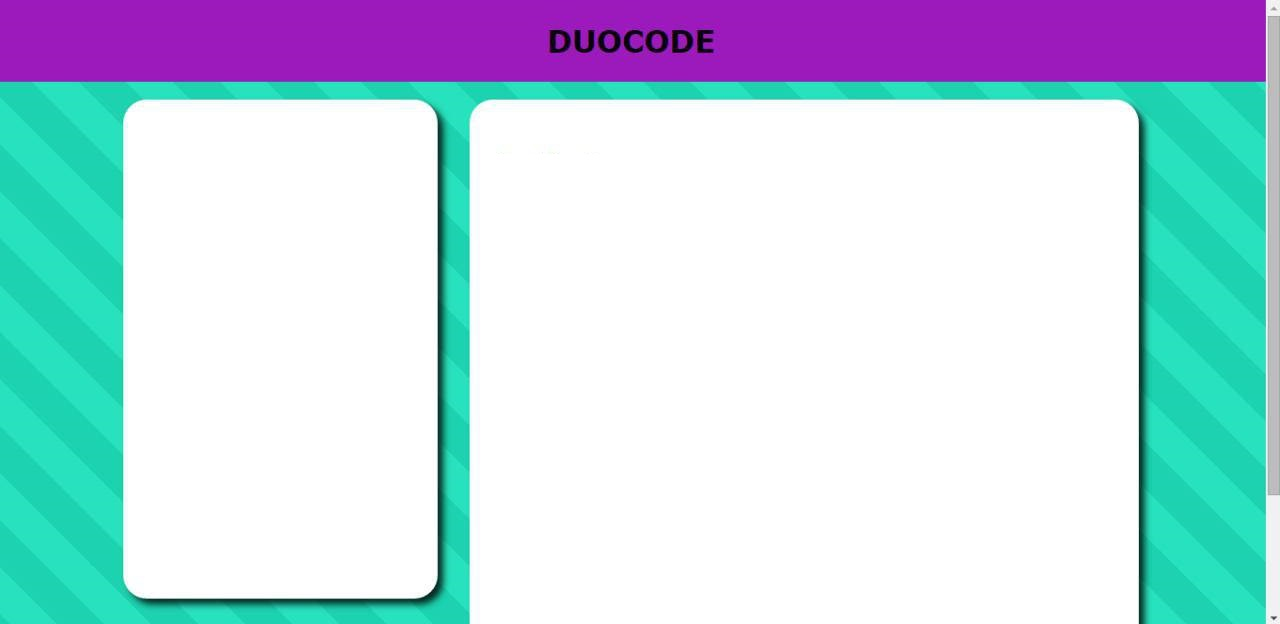
\includegraphics[scale=0.4]{images/color1}}
\end{center}
\end{figure}

\begin{figure}[H]
\begin{center}
\makebox[\textwidth]{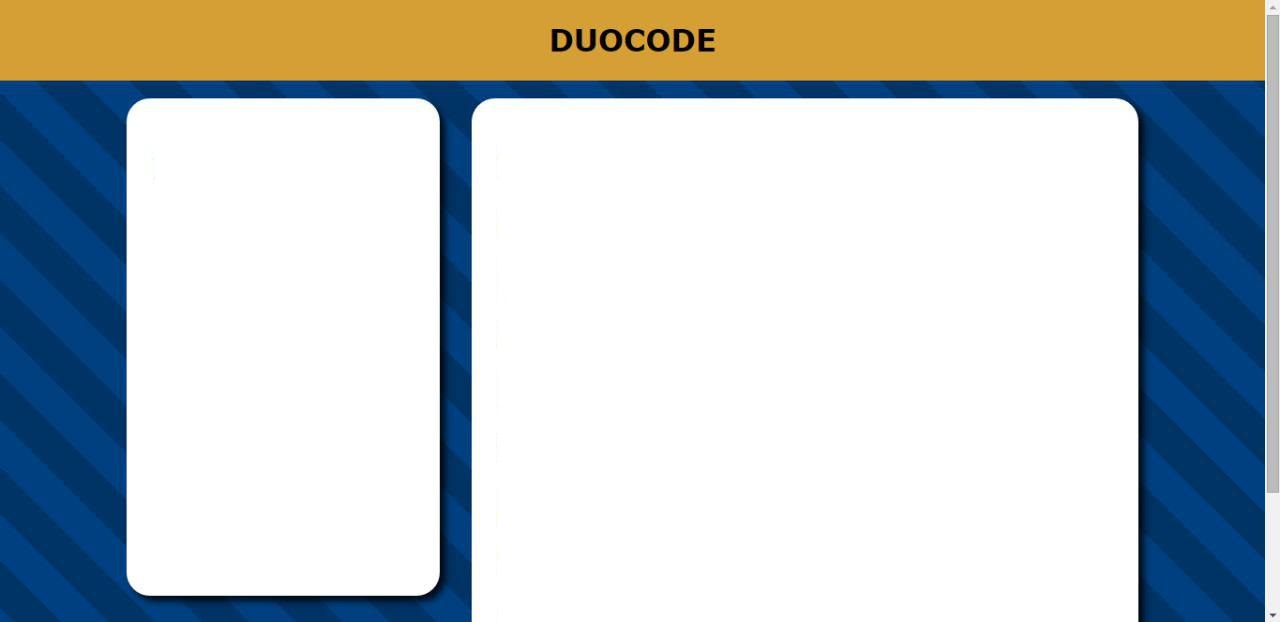
\includegraphics[scale=0.4]{images/color2}}
\end{center}
\end{figure}

Finalmente, pensé en probar con la paleta de colores \texttt{Monokai}, ya que es muy utilizada en programación; esta fue la definitiva.

\item
Incorporé con Bootstrap un pop-up explicativo al iniciar cada lección, el cual está accesible una vez iniciada la sesión por si el usuario quiere volver a verlo. También hice un pop-up explicando qué significa enviar un ejercicio como candidato cuando se da esta opción.

\item
Hice la vista de favoritos del usuario. Para que no saliese demasiada información en esta vista, al principio solo se muestra el título de los ejercicios marcados como favoritos y sus correspondientes lenguajes de programación en los que fueron marcados. Usé la opción \texttt{Collapse} de Bootstrap para mostrar y ocultar el código de los ejercicios cuando el usuario seleccione uno de ellos.

\item
Hice la vista de candidatos de un usuario basándome en la de favoritos para buscar consistencia visual en la web.

\item
Hice la vista de lenguajes que se muestra al entrar en la web. Para que un usuario no pueda elegir el mismo lenguaje de programación en las listas ``Lenguaje que sé'' y ``Lenguaje que quiero aprender'' utilicé AngularJS.

\item
Me encargué de realizar las peticiones al servicio web para saber las lecciones que corresponden a un tema.

\item
Me encargué de realizar las peticiones al servicio web para obtener la información del usuario:

\begin{itemize}
\item
Nombre y foto.
\item
Número de candidatos enviados.
\item
Número de ejercicios marcados como favorito.
\end{itemize}

\item
Me encargué de realizar las peticiones al servicio web para obtener los candidatos de un usuario.

\item
Me encargué de realizar las peticiones al servicio web para obtener los favoritos de un usuario.

\item
Hice que en el pop-up explicativo de las lecciones saliera la información correspondiente.

\item
Añadí la función de iniciar sesión con Google+ y con Facebook mediante la estructura creada por
Julián~F. Calleja da~Silva.

\item
Añadí la función de compartir con Facebook el logro tras superar una lección.

\item
En la memoria me encargué de hacer el resumen y la lista de palabras clave y su traducción al inglés.

\item
En la memoria me encargué de hacer la sección sobre los requisitos y la base de datos
(sección~\ref{sec:req}).

\item
En la memoria me encargué de hacer el manual de usuario (sección~\ref{sec:manual}).

\item
En la memoria me encargué de hacer el apéndice sobre la especificacion de requisitos
(apéndice~\ref{app:req}).

\end{itemize}

\newpage
{\small
\bibliographystyle{abbrv}
\bibliography{tfg_bib}
}


\newpage
\appendix

\section{Especificación de requisitos\label{app:req}}
%!TEX root = memoria_duocode_interfaz.tex

\subsection{localhost/duocode/rest/temas}
\textbf{REQ01 - GET:} No hace falta enviarle ninguna información. Devuelve la lista de todos los temas existentes en modo URL.

\begin{itemize}
\item[•] Response:
\{'temas": ['localhost/duocode/rest/temas/1 ', 'localhost/duocode/rest/temas/2 ']\}
\end{itemize}

\textbf{REQ02 – POST:} Con el post creamos un tema nuevo. Por una parte le pasamos por Payload la información del tema que queremos crear (título, descripción y orden en el que queremos que se muestre): 
\begin{itemize}
\item[•]Payload: 
\{'titulo': 'Bucles', 'descripcion': 'En este tema veremos bucles while y for…', 'orden': '2'\} \vspace{1em}

Por otra parte le enviamos por Header el ID del usuario, el token y el network, que nos sirven para comprobar que el usuario es administrador y tiene permisos para hacer esta operación:
\item[•]Header:
\{'idUsuario': '2', 'token': 'token', 'network': 'network'\}
\vspace{1em}

La respuesta que obtenemos está conformada por “error” e “id”, si la respuesta en el campo “error” es afirmativa significa que algo ha fallado y no ha podido terminar la operación correctamente, en este caso el id será “-1” ya que no ha sido asignado ninguno; si es negativa todo ha ido correctamente y el id será el asignado a este nuevo recurso. Un caso de error podría ser que el usuario no tenga los permisos necesarios.
\item[•]Response:
\{'error': 'no', 'id': '4'\}
\{'error': 'si', 'id': '-1'\}

\end{itemize}

\subsection{localhost/duocode/rest/temas/idTema}

En estos requisitos obtenemos el ID del tema mediante la URL.
\vspace{1em}

\textbf{REQ03 – POST:} Nos devuelve los datos y las lecciones que tiene el tema.

\begin{itemize}
\item[•]Response:
\{'titulo': 'Bucles', 'descripcion': 'En este tema veremos bucles while y for…', 'fechaCreacion': '17/11/2014', 'lecciones': ['localhost/duocode/rest/lecciones/1', 'localhost/duocode/rest/lecciones/2'], 'orden': '2'\}
\end{itemize}

\textbf{REQ04 – PUT:} Modificamos el tema en su totalidad.
\begin{itemize}
\item[•]Payload:
\{'titulo': 'tituloTema', 'descripcion': 'descripcionTema', 'orden': 'int con el orden en el que lo quieres mostrar'\}
\vspace{1em}

Enviamos por Header el ID del usuario, el token y el network, que nos sirven para comprobar que el usuario es administrador y tiene permisos para hacer esta operación:

\item[•]Header: 
\{'idUsuario': '2', 'token': 'token', 'network': 'network'\}
\vspace{1em}

La respuesta que obtenemos está conformada por “error”, en caso afirmativo significa que algo ha fallado y no ha podido terminar la operación correctamente; en caso negativo todo ha ido correctamente. Un caso de error podría ser que el usuario no tenga los permisos necesarios.
\item[•]Response: 
\{'error': 'no'\}
\end{itemize}

\textbf{REQ05 – DELETE:} Borramos el tema completamente. Enviamos por Header el ID del usuario, el token y el network, que nos sirven para comprobar que el usuario es administrador y tiene permisos para hacer esta operación:
\begin{itemize}
\item[•]Header:
\{'idUsuario': '2', 'token': 'token', 'network': 'network'\}
\vspace{1em}

La respuesta que obtenemos está conformada por “error”, en caso afirmativo significa que algo ha fallado y no ha podido terminar la operación correctamente; en caso negativo todo ha ido correctamente. Un caso de error podría ser que el usuario no tenga los permisos necesarios.
\item[•]Response: 
\{'error': 'no'\}
\end{itemize}

\subsection{localhost/duocode/rest/lecciones/}
\textbf{REQ06 – GET:} No hace falta enviarle ninguna información. Devuelve la lista de todas las lecciones existentes en modo URL. 
\begin{itemize}
\item[•]Response:
\{'lecciones': ['localhost/duocode/rest/lecciones/1', 'localhost/duocode/rest/lecciones/2']\}
\end{itemize}

\textbf{REQ07 – POST:} Con el post creamos una nueva lección. Por una parte le pasamos por Payload la información de la lección que queremos crear (título, descripción, explicación que aparecerá al inicio de ésta, orden en el que queremos que se muestre, ID del tema al que pertenecerá, un array de ejercicios que compondrán la lección y otro array de lecciones de las que depende para ser desbloqueada):

\begin{itemize}
\item[•]Payload: 
\{'titulo': 'tituloLeccion', 'descripcion': 'descripcionLeccion', 'explicacion': 'explicacion detallada', 'orden': '4', 'idTema': '1', 'idEjercicios': ['8', '14'], 'leccionesDesbloqueadoras': ['1', '2']\}
\vspace{1em}

Por otra parte le enviamos por Header el ID del usuario, el token y el network, que nos sirven para comprobar que el usuario es administrador y tiene permisos para hacer esta operación:
\item[•]Header: 
\{'idUsuario': '2', 'token': 'token', 'network': 'network'\}
\vspace{1em}

La respuesta que obtenemos está conformada por “error” e “id”, si la respuesta en el campo “error” es afirmativa significa que algo ha fallado y no ha podido terminar la operación correctamente, en este caso el id será “-1” ya que no ha sido asignado ninguno; si es negativa todo ha ido correctamente y el id será el asignado a esta nueva lección. Un caso de error podría ser que el usuario no tenga los permisos necesarios.
\item[•]Response: 
\{'error': 'no', 'id': '3'\}
\{'error': 'si', 'id': '-1'\}
\end{itemize}

\subsection{localhost/duocode/rest/lecciones/idLeccion}
En estos requisitos obtenemos el ID del candidato mediante la URL.
\vspace{1em}


\textbf{REQ08 – GET:} Nos devuelve los datos de la lección, y los ejercicios que tiene la lección.
\begin{itemize}

\item[•]Response:
\{ 'titulo': 'título de la lección (ej. Bucles fácil)', 'descripcion': 'descripción de la lección (ej. primeros bucles para practicar)', 'explicacion': 'explicación detallada', 'fechaCreacion': '17/11/2014', 'ejercicios': ['localhost/duocode/rest/ejercicios/2', 'localhost/duocode/ejercicios/3'], 'leccionesDesbloqueadoras': ['1', '2'], 'orden': '3'\}
\end{itemize}

\textbf{REQ09 – PUT:} Modificamos una lección. Aparte de cambiar los datos de una lección, en este método también podremos marcar como completada la lección para un usuario en un determinado lenguaje por lo que tenemos dos posibles Payloads:

\begin{itemize}
\item[•]Payload para modificar lección:
\{'leccion' : \{'titulo': 'tituloLeccion', 'descripcion': 'descripcionLeccion', 'explicacion':'explicacion detallada', 'idEjercicios': ['1', '2'], 'leccionesDesbloqueadoras': ['2', '3'], 'orden': '2', 'idTema': '1'\} \}

\item[•]
Payload para marcar como lección completada para un usuario:
\{'idUsuarioCompletaLeccion' : '3', 'lenguajeCompletadoLeccion' : 'Java', 'leccion' : \{'titulo': ' tituloLeccion ', 'descripcion': ' descripcionLeccion', 'explicacion':'explicacion detallada', 'idEjercicios': ['1', '2'], 'leccionesDesbloqueadoras': ['2', '3'], 'orden': '2', 'idTema': '1'\} \}

\vspace{1em}
Enviamos por Header el ID del usuario, el token y el network, que nos sirven para comprobar que el usuario es administrador y tiene permisos para hacer esta operación:

\item[•]Header:
\{'idUsuario': '2', 'token': 'token', 'network': 'network'\}
\vspace{1em}

La respuesta que obtenemos está conformada por “error”, en caso afirmativo significa que algo ha fallado y no ha podido terminar la operación correctamente; en caso negativo todo ha ido correctamente. Un caso de error podría ser que el usuario no tenga los permisos necesarios.
\item[•]Response: 
\{'error': 'no'\}
\end{itemize}

\textbf{REQ10 – DELETE:} Borramos la leccion completamente.Enviamos por Header el ID del usuario, el token y el network, que nos sirven para comprobar que el usuario es administrador y tiene permisos para hacer esta operación:
\begin{itemize}

\item[•]
Header: 
\{'idUsuario': '2', 'token': 'token', 'network': 'network'\}
\vspace{1em}

La respuesta que obtenemos está conformada por “error”, en caso afirmativo significa que algo ha fallado y no ha podido terminar la operación correctamente; en caso negativo todo ha ido correctamente. Un caso de error podría ser que el usuario no tenga los permisos necesarios.

\item[•] 
Response: 
\{'error': 'no'\}
\end{itemize}

\subsection{localhost/duocode/rest/ejercicios}
\textbf{REQ11 – GET:} No hace falta enviarle ninguna información. Devuelve la lista de todos los ejercicios existentes en modo URL.

\begin{itemize}
\item[•]
Response: 
\{'ejercicios': ['localhost/duocode/rest/temas/ejercicios/1', 'localhost/duocode/rest/ejercicios/2']\}
\end{itemize}

\textbf{REQ12 – POST:} Creamos un ejercicio nuevo. Por una parte le pasamos el nombre y los enunciados (un mismo ejercicio puede tener varios enunciados porque cada uno corresponde a distintos lenguajes de programación)

\begin{itemize}
\item[•]
Payload: 
\{'nombre': 'nombreDelEjercicio', 'enunciados': [“1”, “2”]\}
\vspace{1em}
Por otra parte le enviamos por Header el ID del usuario, el token y el network, que nos sirven para comprobar que el usuario es administrador y tiene permisos para hacer esta operación:

\item[•]
Header: 
\{'idUsuario': '2', 'token': 'token', 'network': 'network'\}

\vspace{1em}
La respuesta que obtenemos está conformada por “error” e “id”, si la respuesta en el campo “error” es afirmativa significa que algo ha fallado y no ha podido terminar la operación correctamente, en este caso el id será “-1” ya que no ha sido asignado ninguno; si es negativa todo ha ido correctamente y el id será el asignado a este nuevo recurso. Un caso de error podría ser que el usuario no tenga los permisos necesarios.

\item[•]
Response: 
\{'error': 'no', 'id': '4'\}
\{'error': 'si', 'id': '-1'\}
\end{itemize}

\subsection{localhost/duocode/rest/ejercicios/idEjercicio}
En estos requisitos obtenemos el ID del ejercicio mediante la URL.
El get nos devuelve los datos del ejercicio, y los enunciados que tiene el ejercicio (con el id de los lenguajes asociados)
\vspace{1em}

\textbf{REQ13 – GET:} Nos devuelve los datos del ejercicio, los enunciados que tiene y el nombre del lenguaje asociado a cada uno.

\begin{itemize}
\item[•]
Response: \{'nombre': 'nombreDelEjercicio', 'fechaCreacion': '17/11/2014', 'enunciados': [\{'enunciado':'localhost/duocode/rest/enunciados/5', 'nombreLenguaje': 'Java'\}, \{'enunciado':'localhost/duocode/rest/enunciados/8', 'nombreLenguaje': 'C++'\}]\}

\vspace{1em}
Con el delete borramos un ejercicio completamente
\end{itemize}

\textbf{REQ14 – DELETE:} Borramos un ejercicio completamente. Enviamos por Header el ID del usuario, el token y el network, que nos sirven para comprobar que el usuario es administrador y tiene permisos para hacer esta operación:

\begin{itemize}
\item[•]
Header: 
\{'idUsuario': '2', 'token': 'token', 'network': 'network'\}
\vspace{1em}

La respuesta que obtenemos está conformada por “error”, en caso afirmativo significa que algo ha fallado y no ha podido terminar la operación correctamente; en caso negativo todo ha ido correctamente. Un caso de error podría ser que el usuario no tenga los permisos necesarios.
\item[•]
Response: 
\{'error': 'no'\}
\end{itemize}

\subsection{localhost/duocode/rest/enunciados}
\textbf{REQ15 – GET:} No hace falta enviarle ninguna información. Devuelve la lista de todos los enunciados existentes en modo URL. 

\begin{itemize}
\item[•]
Response:
\{'enunciados': [\{'enunciado':'localhost/duocode/rest/enunciados/1', 'nombreLenguaje': 'Java'\}, \{'enunciado':'localhost/duocode/rest/enunciados/2', 'nombreLenguaje': 'C++'\}]\}
\vspace{1em}

\end{itemize}

\textbf{REQ16 – POST:} Creamos un enunciado nuevo. Por una parte le pasamos el lenguaje, el código y el ID del ejercicio correspondiente:

\begin{itemize}
\item[•]
Payload: 
\{'nombreLenguaje': 'Java', 'codigo': 'codigo del enunciado', 'idDelEjercicioQueResuelve': '1'\}
\vspace{1em}

Por otra parte le enviamos por Header el ID del usuario, el token y el network, que nos sirven para comprobar que el usuario es administrador y tiene permisos para hacer esta operación:

\item[•]
Header: 
\{'idUsuario': '2', 'token': 'token', 'network': 'network'\}
\vspace{1em}

La respuesta que obtenemos está conformada por “error” e “id”, si la respuesta en el campo “error” es afirmativa significa que algo ha fallado y no ha podido terminar la operación correctamente, en este caso el id será “-1” ya que no ha sido asignado ninguno; si es negativa todo ha ido correctamente y el id será el asignado a este nuevo enunciado. Un caso de error podría ser que el usuario no tenga los permisos necesarios.

\item[•]
Response: 
\{'error': 'no', 'id': '4'\} 
\{'error': 'si', 'id': '-1'\} 
\end{itemize}

\subsection{localhost/duocode/rest/enunciados/idEnunciado}
En estos requisitos obtenemos el ID del candidato mediante la URL.
\vspace{1em}


\textbf{REQ17 – GET:} Devuelve los datos del enunciado.

\begin{itemize}
\item[•]
Response: 
\{'fechaCreacion': '17/11/2014', 'codigo': 'codigo del enunciado a resolver', 'nombreLenguaje': 'Java', 'idDelEjercicioQueResuelve': '1'\}
\end{itemize}

\textbf{REQ18 – PUT:} Modificamos un enunciado.

\begin{itemize}
\item[•]
Payload: \{'nombreLenguaje': 'Java', 'codigo': 'código del enunciado', 'idDelEjercicioQueResuelve': '1'\}
\vspace{1em}

Enviamos por Header el ID del usuario, el token y el network, que nos sirven para comprobar que el usuario es administrador y tiene permisos para hacer esta operación:
\item[•]
Header: 
\{'idUsuario': '2', 'token': 'token', 'network': 'network'\}
\vspace{1em}

La respuesta que obtenemos está conformada por “error”, en caso afirmativo significa que algo ha fallado y no ha podido terminar la operación correctamente; en caso negativo todo ha ido correctamente. Un caso de error podría ser que el usuario no tenga los permisos necesarios.
\item[•]
Response: 
\{'error': 'no'\}
\end{itemize}

\textbf{REQ19 – DELETE:} Borramos un enunciado completamente. Enviamos por Header el ID del usuario, el token y el network, que nos sirven para comprobar que el usuario es administrador y tiene permisos para hacer esta operación:
\begin{itemize}
\item[•]
Header: 
\{'idUsuario': '2', 'token': 'token', 'network': 'network'\}
\vspace{1em}

La respuesta que obtenemos está conformada por “error”, en caso afirmativo significa que algo ha fallado y no ha podido terminar la operación correctamente; en caso negativo todo ha ido correctamente. Un caso de error podría ser que el usuario no tenga los permisos necesarios.
\item[•]
Response: 
\{'error': 'no'\}
\end{itemize}

\subsection{localhost/duocode/rest/lenguajes/}
\textbf{REQ20 – GET:} No hace falta enviarle ninguna información. Devuelve la lista de todos los lenguajes existentes. 
\begin{itemize}
\item[•]
Response: 
\{'lenguajes': [\{'nombre': 'Java'\}, \{'nombre': 'C++'\}]\}
\end{itemize}

\textbf{REQ21 – POST:} Creamos un lenguaje nuevo. La única información necesaria es el nombre.

\begin{itemize}
\item[•]
Payload: 
\{'nombre': 'Python'\}
\vspace{1em}

Por otra parte le enviamos por Header el ID del usuario, el token y el network, que nos sirven para comprobar que el usuario es administrador y tiene permisos para hacer esta operación:

\item[•]
Header: 
\{'idUsuario': '2', 'token': 'token', 'network': 'network'\}
\vspace{1em}

La respuesta que obtenemos está conformada por “error” y “nombreConfirmacion”, si la respuesta en el campo “error” es afirmativa significa que algo ha fallado y no ha podido terminar la operación correctamente; si es negativa todo ha ido correctamente y el “nombreConfirmacion” será el asignado a este nuevo lenguaje. Un caso de error podría ser que el usuario no tenga los permisos necesarios.

\item[•]
Response: 
\{'error': 'no', ' nombreConfirmacion ': 'Python'\}

\end{itemize}

\subsection{localhost/duocode/rest/candidatos/}
\textbf{REQ22 – GET:} No hace falta enviarle ninguna información. Devuelve la lista de todos los candidatos existentes en modo URL. 

\begin{itemize}
\item[•]
Response: 
\{'candidatos': ['localhost/duocode/rest/candidatos/1', 'localhost/duocode/rest/candidatos/2']\}
\end{itemize}

\textbf{REQ23 – POST:} Generamos un nuevo candidato, y le asociamos el usuario que lo ha creado. Por un lado le enviamos el código del candidato, el ID del ejercicio que resuelve, el lenguaje en el que está escrito el candidato y el lenguaje del enunciado:
\begin{itemize}
\item[•]
Payload: 
\{'codigo': 'codigoDelCandidato', 'idEjercicio': '4', 'nombreLenguajeDestino': 'Java', 'nombreLenguajeOrigen': 'C++'\}
\vspace{1em}

Por otra parte le enviamos por Header el ID del usuario, el token y el network, que nos sirven para saber qué usuario es el que ha enviado el candidato:
\item[•]
Header: 
\{'idUsuario': '2', 'token': 'token', 'network': 'network'\}
\vspace{1em}

La respuesta que obtenemos está conformada por “error” e “idCandidato”, si la respuesta en el campo “error” es afirmativa significa que algo ha fallado y no ha podido terminar la operación correctamente, en este caso el id será “-1” ya que no ha sido asignado ninguno; si es negativa todo ha ido correctamente y el id será el asignado a este nuevo enunciado. 
\item[•]
Response: 
\{'error': 'no', 'id': '4'\}
\end{itemize}

\subsection{localhost/duocode/rest/candidatos/idCandidato}
En estos requisitos obtenemos el ID del candidato mediante la URL.
\vspace{1em}

\textbf{REQ24 – GET:} Devuelve los datos de un candidato, incluidos los votos que tiene.

\begin{itemize}
\item[•]
Response: 
\{'idEjercicio': 'localhost/duocode/rest/ejercicios/4', 'nombreLenguajeOrigen' : 'Java', 'nombreLenguajeDestino : 'C++', 'codigo' : 'codigo del candidato', 'idUsuarioCreador' : '2', 'fechaCreacion': '17/11/2014', 'votos': [ \{idUsuarioVoto':'8', 'voto': 'pos'\}, \{idUsuarioVoto':'5', 'voto': 'neg'\} ] \}
\end{itemize}

\textbf{REQ25 – PUT:} Excepcionalmente no modificará todo el candidato, sino que servirá para que un usuario pueda votar, modificar el voto o eliminarlo (si se vuelve a votar positivo o negativo el voto se anula). Se envía el ID del usuario y el voto (1 si es positivo y 0 si es negativo).

\begin{itemize}
\item[•]
Payload: 
\{'votar': \{'idUsuario': 6, 'voto': 1\}\}
\vspace{1em}

La respuesta que obtenemos está conformada por 'error', en caso afirmativo significa que algo ha fallado y no ha podido terminar la operación correctamente; en caso negativo todo ha ido correctamente. 
\item[•]
Response: 
\{'error': 'no'\}
\end{itemize}

\textbf{REQ26 – DELETE:} Borramos un candidato completamente.

\begin{itemize}
\item[•]
Header: 
\{'idUsuario': '2', 'token': 'token', 'network': 'network'\}
\vspace{1em}

La respuesta que obtenemos está conformada por “error”, en caso afirmativo significa que algo ha fallado y no ha podido terminar la operación correctamente; en caso negativo todo ha ido correctamente. Un caso de error podría ser que el usuario no tenga los permisos necesarios.

\item[•]
Response: 
\{'error': 'no'\}
\end{itemize}

\subsection{localhost/duocode/rest/usuarios/}
El GET devuelve todos los usuarios, solo si lo pide un administrador (esta petición va con el ID de un usuario administrador y el token)
\textbf{REQ27 – GET:} Devuelve todos los usuarios. A diferencia de otros, este GET sólo lo puede hacer un administrador por lo que necesitamos nuevamente del Header.

\begin{itemize}
\item[•]
Header:
\{'idUsuario': '2', 'token': 'token', 'network': 'network'\}
\vspace{1em}

La respuesta que obtenemos está conformada por “error” y la lista de usuarios. Si “error” tiene una respuesta afirmativa, significa que algo ha fallado y no ha podido terminar la operación correctamente; en caso negativo todo ha ido correctamente y muestra la lista de usuarios mediante su URL. Un caso de error podría ser que el usuario no tenga los permisos necesarios.

\item[•]
Response: 
\{'error': 'no”, 'usuarios' : ['localhost/duocode/rest/usuario/1', 'localhost/duocode/rest/usuario/2'] \}
\end{itemize}

\subsection{localhost/duocode/rest/usuarios/idUsuario}
En estos requisitos obtenemos el ID del candidato mediante la URL.
\vspace{1em}

\textbf{REQ28 – GET:} Devuelve la información asociada a un usuario. Enviamos por Header el ID del usuario, el token y el network, que nos sirven para comprobar que el usuario que accede es el mismo del que se da la información:

\begin{itemize}
\item[•]
Header: 
\{'idUsuario': '2', 'token': 'token', 'network': 'network'\}
\vspace{1em}

La respuesta es la información detallada de toda la sesión del usuario
\item[•]
Response: \{'nick' : 'nickDelUsuairo',
'leccionesCompletadas' : ['localhost/duocode/rest/lecciones/1', 'localhost/duocode/rest/lecciones/2'],
'favoritos': [\{'ejercicio' : 'localhost/duocode/rest/ejercicios/5', 'nombreLenguajeOrigien': 'Java', 'nombreLenguajeDestino': 'C++'\}, \{'ejercicio' : 'localhost/duocode/rest/ejercicios/7', 'nombreLenguajeOrigien': 'Python', 'nombreLenguajeDestino': 'C++'\}],
'historialEjercicios' : [\{'idEnvio': '1', 'ejercicio' : 'localhost/duocode/rest/ejercicios/4', 'nombreLenguajeOrigien': 'Java', 'nombreLenguajeDestino': 'C++', 'codigo': 'codigo enviado', 'fecha': '17/11/2014', 'puntuacion' : '2'\}, \{'idEnvio': '2', 'ejercicio' : 'localhost/duocode/rest/ejercicios/9', 'nombreLenguajeOrigien': 'Python', 'nombreLenguajeDestino': 'Perl', 'codigo': 'codigo enviado', 'fecha': '18/11/2014', 'puntuacion' : '7'\}],
'candidatosPropuestos': ['localhost/duocode/rest/candidatos/18', 'localhost/duocode/rest/candidatos/23'] \}
\end{itemize}

\textbf{REQ29 – DELETE}: Borramos un usuario completamente.
Enviamos por Header el ID del usuario, el token y el network, que nos sirven para comprobar que el usuario es administrador y tiene permisos para hacer esta operación:

\begin{itemize}
\item[•]
Header: 
\{'idUsuario': '2', 'token': 'token', 'network': 'network'\}
\vspace{1em}

La respuesta que obtenemos está conformada por “error”, en caso afirmativo significa que algo ha fallado y no ha podido terminar la operación correctamente; en caso negativo todo ha ido correctamente. Un caso de error podría ser que el usuario no tenga los permisos necesarios.

\item[•]
Response: 
\{'error': 'no'\}
\end{itemize}

\subsection{localhost/duocode/rest/envios}
\textbf{REQ30 – GET}: Devuelve todos los envíos para que un administrador pueda tener información de ellos. Como sólo puede tener acceso a esto el administrador, es necesaria la siguiente información:

\begin{itemize}
\item[•]
Header: 
\{'idUsuario': '2', 'token': 'token', 'network': 'network'\}
\vspace{1em}

La respuesta se compone de usuarios con historiales de ejercicios.

\item[•]
Response: \{ 'envios' : [ \{'idUsuario': '1', 'historialEjercicios' : [\{'idEnvio': '1', 'ejercicio' : 'localhost/duocode/rest/ejercicios/5', 'nombreLenguajeOrigien': 'Java', 'nombreLenguajeDestino': 'C++', 'codigo': 'codigo enviado', 'fecha': '17/11/2014', 'puntuacion' : '2'\}, \{'idEnvio': '2', 'ejercicio' : 'localhost/duocode/rest/ejercicios/7', 'nombreLenguajeOrigien': 'Python', 'nombreLenguajeDestino': 'Perl', 'codigo': 'codigo enviado', 'fecha': '18/11/2014', 'puntuacion' : '7'\}]\},
\{'idUsuario': '4', 'historialEjercicios' : [\{'idEnvio': '1', 'ejercicio' : 'localhost/duocode/rest/ejercicios/6', 'nombreLenguajeOrigien': 'Java', 'nombreLenguajeDestino': 'C++', 'codigo': 'codigo enviado', 'fecha': '17/11/2014', 'puntuacion' : '2'\}, \{'idEnvio': '2', 'ejercicio' : 'localhost/duocode/rest/ejercicios/5', 'nombreLenguajeOrigien': 'Python', 'nombreLenguajeDestino': 'Perl', 'codigo': 'código enviado', 'fecha': '18/11/2014', 'puntuacion' : '7'\}]\} ] \}
\end{itemize}

\textbf{REQ31 – PUT:} Corregimos un ejercicio, y también se comprobará si se ha completado la lección y en caso afirmativo se marcará como completada en la BD. Por una parte enviamos la URL del ejercicio, el lenguaje del enunciado, el lenguaje de la solución y el código.

\begin{itemize}
\item[•]
Payload: 
\{'ejercicio': 'localhost/duocode/rest/ejercicios/idEjercicio1', 'nombreLenguajeOrigien': 'Java', 'nombreLenguajeDestino': 'C++', 'codigo': 'codigo enviado en el lenguaje de destino'\} 
\vspace{1em}

Por otra parte enviamos el idUsuaro, token y network para comprobar que el usuario que envía el ejercicio para corregir es el que tiene la sesión iniciada.
\item[•]
Header: \{'idUsuario': 'idDelUsuario', 'token': 'token', 'network': 'network'\}
\vspace{1em}

La respuesta que obtenemos está conformada por “error” y “puntuacion”. Si “error” tiene un valor afirmativo significa que algo ha fallado y no ha podido terminar la operación correctamente; en caso negativo todo ha ido correctamente y devuelve la puntuación que ha obtenido el ejercicio al ser corregido. Un caso de error podría ser que el usuario no coincida.
\item[•]
Response: \{'error': 'no', 'puntuacion': '2'\}
\end{itemize}


\newpage
\section{Manual de instalación\label{app:manual}}
En este apartado se detallan los pasos a seguir para tener instalado \textbf{DuoCode} en un sistema \textit{Linux}, con el fin de poder trabajar directamente con los ficheros fuentes y extender el proyecto. La dirección donde podemos descargar todo el código es \url{https://github.com/jucallej/DuoCode.git}.

El software necesario para trabajar con el proyecto se especifica a continuación.

\begin{itemize}
\item \textbf{Requisitos generales}
\begin{itemize}
\item Java 7.
\item Git.
\item Navegador Web - Google Chrome.
\end{itemize}
\end{itemize}
\begin{itemize}
\item \textbf{Requisitos para el Servicio Web}
\begin{itemize}
\item Xampp.
\item Tomcat 8.0.
\item NetBeans 8.0.
\end{itemize}
\end{itemize}
\begin{itemize}
\item \textbf{Requisitos para el Front-End}

\begin{itemize}
\item Soporte SSL en Xampp y Tomcat.
\end{itemize}
\end{itemize}
\begin{itemize}
\item \textbf{Requisitos para la Aplicación móvil}
\begin{itemize}
\item Node.Js 0.10.X.
\item Phonegap 5.0.0.
\item Eclipse Luna con plugin para Android.
\end{itemize}
\end{itemize}

\subsection{Instalación de desarrollador}

Es importante seguir el orden de instalación que aparece a continuación para no tener problemas de dependencias entre programas. 

\begin{itemize}
\item \textbf{Java}

En primer lugar necesitamos tener instalada una versión de Java. La forma más sencilla es acceder a la web \url{http://www.java.com/es/} y descargar la última versión.

Es posible usar el siguiente comando en el termina:
{\codesize
\begin{verbatim}
$ sudo apt-get install openjdk-7-jdk openjdk-7-jre
\end{verbatim}
}


\item \textbf{Git}

Para poder descargar todos los ficheros fuentes del proyecto es necesario tener un cliente Git instalado y configurado.

Una opción es acceder a la web \url{http://git-scm.com/downloads/guis} y elegir el cliente que queramos. 

Es posible usar el siguiente comando en el termina:

{\codesize
\begin{verbatim}
$ sudo apt-get install git
\end{verbatim}
}

Una vez instalado git podemos clonar el proyecto \textbf{DuoCode} y obtener una copia en nuestro sistema. Si trabajas con un cliente gráfico simplemente hay que pinchar en el botón \textit{clone} y escribir la dirección del repositorio \url{https://github.com/jucallej/DuoCode.git}.

También podemos clonar el proyecto directamente desde la línea de comandos:
{\codesize
\begin{verbatim}
$ git clone https://github.com/jucallej/DuoCode.git
\end{verbatim}
}


\item \textbf{Google Chrome}

Cualquier navegador es válido pero Chrome cuenta con un plugin (Advance Rest Client) que es necesario para hacer pruebas con el servicio REST. Para instalar el navegador accedemos a la web de Chrome \url{https://www.google.es/chrome/} y pinchamos en el botón de descarga.

Es posible usar el siguiente comando en el termina:
{\codesize
\begin{verbatim}
$ sudo apt-get install google-chrome-stable
\end{verbatim}
}



\item \textbf{XAMPP}

Es necesario tener instalado un servidor local. XAMPP nos proporciona una base de datos MySQL y un servidor Apache.
Para instalarlo solo hay que acceder a la web \url{https://www.apachefriends.org/index.html} y descargar la última versión disponible.


Una vez instalado y funcionando accedemos a \url{http://localhost/phpmyadmin} para importar la Base de datos.
Creamos una Base de datos nueva con el nombre `Duocode', la seleccionamos e importamos el archivo 'Duocode.sql' para que nos cree las tablas y cargue la información del proyecto.


En la carpeta \textit{`htdocs'}, que se encuentra dentro de la carpeta del servidor XAMPP, es donde tenemos que poner la parte del front-end.
Copiamos la carpeta \textit{`duocode'} que contiene el \textit{`index.html'} y todos los scripts y la pegamos en \textit{`htdocs'}.
Podemos probar el funcionamiento accediendo a la dirección \url{`http://localhost/duocode'}.



\item \textbf{Tomcat}

Para el servicio web REST necesitamos tener instalado Tomcat 8.0 o superior. Para ello, accedemos a la web \url{http://tomcat.apache.org/download-80.cgi} (para la versión 8.0), descargamos la última versión para nuestro sistema operativo y lo descomprimimos.



\item \textbf{NetBeans}

El IDE que se ha usado para desarrollar el proyecto es NetBeans 8.0. Nos permite integrar el sistema de control de versiones \textit{Git} y los servidores. Se puede descargar desde la web \url{https://netbeans.org/downloads/}.

Una vez instalado importamos el proyecto descargado desde el Git y seleccionamos el servidor con el que queremos que funcione, en nuestro caso será el Tomcat descargado anteriormente.

Las bibliotecas necesarias se importan de manera automática una vez que hemos cargado el proyecto en NetBeans.

\item \textbf{Certificados SSL}

Para que tanto el front-end como el servicio web funcionen con \textit{https} es necesario activar SSL en los servidores \textit{Tomcat} y \textit{Apache} del XAMPP.

Hemos creado nuestros propios certificados SSL y se pueden encontrar en la carpeta \textit{duocode/certificados}. Ña contraseña es \textit{complutense}.

Tomcat lo podemos configurar gracias al archivo \textit{server.xml} encontrado en /apache-tomcat-8.0.21/conf/server.xml.
Lo abrimos y dentro del elemento:
{\codesize
\begin{verbatim}
 < Service name = 'Catalina' >  
\end{verbatim}
}
pegamos estas líneas de código (cambiando la ruta del proyecto):

{\codesize
\begin{verbatim}
<Connector port="8443" protocol="org.apache.coyote.http11.Http11NioProtocol"
               maxThreads="150" SSLEnabled="true" scheme="https" secure="true"
               clientAuth="false" sslProtocol="TLS"
           keystoreType="PKCS12"
           keystoreFile="{Ruta al repositorio}\DuoCode\duocode\certificados\mycert.p12" keystorePass="contraseña"/>
\end{verbatim}
}

Para configurar el server Apache que nos proporciona XAMPP primero tenemos que poner los archivos \textit{`mars-server.crt', `mars-server.key'} en la siguiente ruta:

\begin{itemize}


\item \textit{'/opt/lampp/etc/ssl.crt/'} los ficheros con la extensión .crt.

\item \textit{'/opt/lampp/etc/ssl.key/'} el fichero con la extensión .key.

\end{itemize}

Una vez tenemos los certificados y la clave en las rutas adecuadas editamos el fichero \textit{httpd-ssl.conf}. Dependiendo de la versión puede tener un aspecto u otro, en nuestro caso hemos definido un nuevo VirtualHost con la siguiente configuración.

{\codesize
\begin{verbatim}
<VirtualHost _default_:443>

DocumentRoot "/opt/lampp/htdocs"
ServerName localhost:443
ServerAdmin you@example.com
ErrorLog "/opt/lampp/logs/error_log"
TransferLog "/opt/lampp/logs/access_log"

SSLEngine on

SSLCertificateFile "/opt/lampp/etc/ssl.crt/mars-server.crt"
SSLCertificateKeyFile "/opt/lampp/etc/ssl.key/mars-server.key"
SSLCertificateChainFile "/opt/lampp/etc/ssl.crt/my-ca.crt"

SSLCACertificateFile "/opt/lampp/etc/ssl.crt/my-ca.crt"

<FilesMatch "\.(cgi|shtml|phtml|php)$">
    SSLOptions +StdEnvVars
</FilesMatch>
<Directory "/opt/lampp/cgi-bin">
    SSLOptions +StdEnvVars
</Directory>

BrowserMatch "MSIE [2-5]" \
         nokeepalive ssl-unclean-shutdown \
         downgrade-1.0 force-response-1.0

CustomLog "/opt/lampp/logs/ssl_request_log" \
          "%t %h %{SSL_PROTOCOL}x %{SSL_CIPHER}x \"%r\" %b"

<Directory "/opt/lampp/htdocs">
        Options Indexes
        AllowOverride None
        Allow from from all
        Order allow,deny
</Directory>

</VirtualHost>
\end{verbatim}
}

Una vez configurado podemos acceder a la dirección \url{https://localhost/duocode}, aunque nos saldrá un mensaje indicando que el certificado no está verificado (es un certificado que hemos creado nosotros) así que lo añadimos como excepción y ya tenemos \textbf{DuoCode} instalado.


\item \textbf{Node.js}

Para poder trabajar con PhoneGap - Cordova es necesario tener instalado Node.js en nuestro equipo. Podemos hacerlo descargándolo desde la web \url{`https://nodejs.org/'} o directamente desde un terminal:

{\codesize
\begin{verbatim}
$ sudo add-apt-repository ppa:chris-lea/node.js
$ sudo apt-get update
$ sudo apt-get install nodejs
\end{verbatim}
}

Es necesario que la versión sea 0.8+. Podemos comprobarlo tecleando desde el terminal: 

{\codesize
\begin{verbatim}
$ node -v
\end{verbatim}
}

\item \textbf{PhoneGap}

PhoneGap nos sirve para crear una app móvil desde el HTML5, CSS y JS de nuestro proyecto. Para instalarlo podemos descargarlo desde la web \url{http://phonegap.com} o directamente desde un terminal:

{\codesize
\begin{verbatim}
$ npm install -g phonegap
\end{verbatim}
}

\item \textbf{Eclipse y Android SDK}

Gracias al plugin de Android podemos usar Eclipse como IDE para probar la app móvil de DuoCode. Instalamos la última versión de Eclipse descargándolo desde la web \url{http://eclipse.org}.

Una vez descargado lo abrimos y vamos a añadir el plugin para Android.
Pinchamos en \textbf{help - Install New Software} y añadimos la siguiente URL \url{https://dl-ssl.google.com/android/eclipse/} y seleccionamos \textbf{next} hasta completar la instalación.

Reiniciamos Eclipse y tenemos que especificar la dirección del \textbf{Android SDK} que acabamos de descargar para que se actualice y tener Eclipse listo.

Podemos importar la carpeta del proyecto que encontramos en DuoCode y probarlo con el emulador seleccionando la carpeta del proyecto y pulsando sobre \textit{`Run'}.

\end{itemize}

\subsection{Desplegado modo desarrollador}

Finalmente, una vez instalado y configurado todo, podemos desplegar y trabajar sobre el proyecto local.

Tenemos que seguir una serie de pasos que se detallan a continuación:

\begin{itemize}

\item \textbf{Arranque de XAMPP}

Para arrancar el servidor Apache y tener acceso a la Base de datos es necesario que \textit{XAMPP} esté funcionando. Para ello abrimos un terminal, nos posicionamos en la carpeta donde se haya instalado \textit{`/opt/lampp/'} y escribimos el siguiente comando:
{\codesize
\begin{verbatim}
$ ./xampp start
\end{verbatim}
}
Es posible que se quede parado mientras intenta arrancar el servidor Apache porque necesite la contraseña del certificado. Si esto ocurre escribimos en el terminal \textit{`complutense'} y pulsamos Enter.



\item \textbf{Despliegue del servicio REST}

Para desplegar el servicio REST abrimos Netbeans y seleccionamos el proyecto DuoCode que importamos durante la instalación. Accedemos a \textit{Run} - \textit{Build} y después pulsamos con el botón derecho del ratón sobre la carpeta del proyecto y seleccionamos \textit{Deploy}.

Con estos pasos conseguimos que el servidor Tomcat se inicie y se despliegue el servicio REST.

\item \textbf{Acceso a DuoCode}

Si no se ha producido ningún problema durante la instalación y el despliegue podemos acceder a la web \url{https://localhost/duocode} y probar la aplicación.

\end{itemize}
}
\appendix


%\input{divide_y_venceras}

\end{document}
